\documentclass[a4paper,pdftex,10pt]{article}
\usepackage[margin=2.5cm,nohead]{geometry}
\usepackage[utf8]{inputenc}
\usepackage[T1]{fontenc} 
\usepackage[english,slovene]{babel} 
\usepackage{amsmath,amsfonts,amsthm,amssymb,mathrsfs,empheq} % Math packages
\usepackage{mathtools}
\usepackage{dsfont}
\usepackage{wrapfig}
\usepackage[pdftex]{graphicx}
%\usepackage{makeidx}
\usepackage{url}
\usepackage{caption}
\usepackage{subcaption}
\usepackage{tabularx}
\usepackage{float}

\usepackage[version=3]{mhchem} %kemija

\DeclarePairedDelimiter{\evdel}{\langle}{\rangle}   %pricakovana vrednost


\renewcommand{\vec}[1]{\boldsymbol{\mathbf{#1}}}                                        
\newcommand{\ihat}[0]{\boldsymbol{\mathbf{\oldhat{\textbf{\i}}}}} % pokončna j in i (j i n i
\newcommand{\iu}{{i\mkern1mu}}	    %imaginarno število
\DeclarePairedDelimiterX{\norm}[1]{\lVert}{\rVert}{#1} %norma

\usepackage{fancyhdr} % Custom headers and footers
\pagestyle{fancyplain} % Makes all pages in the document conform to the custom headers and footers
\fancyhead{} % No page header - if you want one, create it in the same way as the footers below
\fancyfoot[L]{} % Empty left footer
\fancyfoot[C]{} % Empty center footer
\fancyfoot[R]{\thepage} % Page numbering for right footer
\renewcommand{\headrulewidth}{0pt} % Remove header underlines
\renewcommand{\footrulewidth}{0pt} % Remove footer underlines
\setlength{\headheight}{13.6pt} % Customize the height of the header

%\numberwithin{equation}{section} % Number equations within sections (i.e. 1.1, 1.2, 2.1, 2.2 instead of 1, 2, 3, 4)
\numberwithin{figure}{section} % Number figures within sections (i.e. 1.1, 1.2, 2.1, 2.2 instead of 1, 2, 3, 4)
%\numberwithin{table}{section} % Number tables within sections (i.e. 1.1, 1.2, 2.1, 2.2 instead of 1, 2, 3, 4)

\setlength\parindent{0pt} % Removes all indentation from paragraphs - comment this line for an assignment with lots of text

%----------------------------------------------------------------------------------------
%	TITLE SECTION
%----------------------------------------------------------------------------------------

\newcommand{\horrule}[1]{\rule{\linewidth}{#1}} % Create horizontal rule command with 1 argument of height

\title{	
\normalfont \normalsize 
\textsc{Modelska analiza 1} \\ [25pt] % Your university, school and/or department name(s)
%\horrule{0.2pt} \\[0.4cm] % Thin top horizontal rule
\huge 8. naloga - Metropolisov algoritem\\ % The assignment title
%\horrule{0.2pt} \\[0.5cm] % Thick bottom horizontal rule
}

\author{Tina Klobas} % Your name

\date{\normalsize\today} % Today's date or a custom date

\begin{document}

\maketitle % Print the title

\section{Opis problema}
Pri Metropolis-Hastingovem algoritmu uporabljamo metodo Monte Carlo, da zaporedoma žrebamo 
vzorce s~poljubno verjetnostno porazdelitvijo. Tako lahko dobimo približke porazdelitvenih
funkcij (oziroma histograme s~tako porazdelitvijo) ali izračunamo integrale (pričakovane
vrednosti po izbrani porazdelitvi). Metropolisov algoritem je poseben primer omenjenega
algoritma v~katerem imamo simetrično porazdelitveno funkcijo. Splošen potek takega
algoritma:
\begin{enumerate}
    \item izberemo začetek spehoda $x_0$ in verjetnostno gostoto $\rho (x|y)$, po
	kateri hočemo vzorčiti, in ki izbere kandidata za naslednjo vrednost $x$ pri 
	trenutni vrednosti $y$ (za Metropolisov algoritem je ta funkcija simetrična - 
	$\rho (x|y) = \rho (y|x)$).
    \item Na koraku $t+1$:
	\begin{enumerate}
	    \item po gostoti $\rho (x'|x_t)$ generiramo naključnega kandidata $x'$ in 
		izračunamo verjetnost \emph{sprejema}:
		\begin{equation}
		    \alpha = \mathrm{min} \, \left\{
			1, \, \frac{P(x')}{P(x_t)} \, \frac{R(x_t|x')}{R(x'|x_t)} \right\},
		\end{equation}
		kjer je $R(z)$ \emph{predlagana} verjetnost (po gostoti $\rho (z)$),
		$P(z)$ pa verjetnost za izbrano stanje Markove verige.
	    \item Izberemo naključno število $\gamma$ z~intervala $[0,1]$ in če je $\alpha 
		> \gamma $ zavrnemo kandidata $x'$ in obdržimo prejšnje stanje $x_{t+1} = 
		x_t$, če pa velja $\alpha \leq \gamma$ obdržimo kandidata in novo stanje je
		$x_{t+1} = x'$.
	\end{enumerate}
\end{enumerate}
Poseben primer je tudi neodvisen Metropolisov algoritem, kjer trenutno stanje modela ni 
odvisno od predhodnega stanja. Tako na vsakem koraku žrebamo kandidata po porazdelitvi 
$x' \sim \, \rho(x)$, verjetnost sprejema pa je v~tem primeru
\begin{equation} 
    \alpha = \mathrm{min} \, \left\{ 1, \, \frac{P(x')}{P(x_t)} \, \frac{R(x_t)}{R(x')} 
    \right\}.
\end{equation}

\pagebreak
%----------------------------------------------------------------------------------------
%	PROBLEM 1
%----------------------------------------------------------------------------------------
\section{Molekularna verižnica}
Nitkasta molekula sestavljena iz 17 členkov je obešena na obeh koncih. Vsak členek se lahko
povesi od začetnega ničelnega nivoja na poljubnega od 19 nivojev in si s~zmanjša potencialno
energijo. Po drugi strani s~premikom spremenimo tudi prožnostno energijo med sosedi. 
Določiti želimo ravnovesno energijo v~odvisnosti od temperature. Na vsakem koraku $t$ 
spremenimo položaj naključnega členka v~verigi. \\
Z~vektorjem $\vec{h}$ si beležimo višine členkov, za katere velja $h_0 = h_{17} = 0$.
Celotna energija $E$ je tako sestavljena iz potencialnega
\begin{equation}
    E_{\text{pot}} = \sum_{i=1}^{17} \alpha h_i 
\end{equation}
in prožnostnega prispevka
\begin{equation}
    E_{\text{pr}} = \sum_{i=1}^{16} \frac{1}{2} (h_{i+1} -h_i)^2.
\end{equation}
Na vsakem koraku $t$ spremenimo položaj naključnega členka $h_i$ In imamo tako kandidata
$h'_i = h_i + \Delta$, kjer je naključen premik izbran tako, da je členek po premiku še 
zmeraj znotraj nivojskega sistema. Sprememba energije je potem:
\begin{equation}
    \Delta E = E' - E = \Delta \left[ \, \alpha + 2 h_i + \Delta - h_{i+1} - h_{i-1} 
    \, \right]
\end{equation}
Predlagana verjetnost $R$ je v~tem primeru $R(h_i) = 1/N$ in je enaka za vsak člen verige.
Verjetnost, da je model v~stanju z~energijo $E$ pa je odvisen on temperature in je enak 
$P(E) = \mathrm{e}^{- \beta E}$ kjer je $\beta = 1/k_{\mathrm{B}} T $. Verjetnost sprejetja
je tako
\begin{equation}
    \alpha = \text{min} \left\{ 1, \mathrm{e}^{- \beta \Delta E}  \right\}.
\end{equation}
Izžrebamo naljučno število $\zeta \sim U[0,1]$ in če velja $\zeta \leq \mathrm{e}^{- \beta 
\Delta E}$ sprejmemo novo stanje in naredimo premik $h_{i+1} = h'_i$, sicer pa premik
zavrnemo in $h_{i+1} = h_i$. Vidimo, da bo za vsak $\Delta E < 0$ eksponentna funkcija
vedno večja od $1$, torej bo $\alpha=1$ in so vsi premiki, ki sistemu zmanjšajo energijo,
ugodni. V~limiti, ko gre $T \rightarrow \infty$ gre eksponentna funkcija proti $1$ in 
sprejmemo vse premike, v drugem primeru ko gre $T \rightarrow 0$ pa sprejmemo le tiste
premike, ki znižajo energijo.

\subsection{Rezultati}
Nivoje lahko poljubno naredimo \emph{diskretne} (samo celoštevilska stanja) ali 
\emph{zvezne} (dodamo tudi racionalna števila), prav tako lahko omejimo premik na vsakem 
koraku. Oglejmo si tri različne primere in kako se razlikujejo končna stanja takih 
algoritmov:
\begin{enumerate}
    \item diskretni nivoji z~dovoljenim preskomom le na sosednji ravni: sprememba 
	višine je $\Delta h =  (-1)^{2 \delta + 1}$, kjer je $\delta \in \mathds{Z}^+ \! 
	\cup \!  \{0\}$ in jo naključno žrebamo na vsakem koraku. Sprememba energije je 
	potem: 
	\begin{equation} 
	    \Delta E = E' - E = 1 + (-1)^{2 \delta_i + 1} \left[ \, \xi + k \left(2 h_i - 
	    h_{i+1} - h_{i-1} \right) \, \right].
	\end{equation}
    \item diskretni nivoji s~poljubnim premikom in 
    \item zvezni nivoji s~poljubnim premikom.
\end{enumerate}

\begin{figure}    
    \centering
    \resizebox{0.75\linewidth}{!}{% GNUPLOT: LaTeX picture with Postscript
\begingroup
  \makeatletter
  \providecommand\color[2][]{%
    \GenericError{(gnuplot) \space\space\space\@spaces}{%
      Package color not loaded in conjunction with
      terminal option `colourtext'%
    }{See the gnuplot documentation for explanation.%
    }{Either use 'blacktext' in gnuplot or load the package
      color.sty in LaTeX.}%
    \renewcommand\color[2][]{}%
  }%
  \providecommand\includegraphics[2][]{%
    \GenericError{(gnuplot) \space\space\space\@spaces}{%
      Package graphicx or graphics not loaded%
    }{See the gnuplot documentation for explanation.%
    }{The gnuplot epslatex terminal needs graphicx.sty or graphics.sty.}%
    \renewcommand\includegraphics[2][]{}%
  }%
  \providecommand\rotatebox[2]{#2}%
  \@ifundefined{ifGPcolor}{%
    \newif\ifGPcolor
    \GPcolortrue
  }{}%
  \@ifundefined{ifGPblacktext}{%
    \newif\ifGPblacktext
    \GPblacktexttrue
  }{}%
  % define a \g@addto@macro without @ in the name:
  \let\gplgaddtomacro\g@addto@macro
  % define empty templates for all commands taking text:
  \gdef\gplbacktext{}%
  \gdef\gplfronttext{}%
  \makeatother
  \ifGPblacktext
    % no textcolor at all
    \def\colorrgb#1{}%
    \def\colorgray#1{}%
  \else
    % gray or color?
    \ifGPcolor
      \def\colorrgb#1{\color[rgb]{#1}}%
      \def\colorgray#1{\color[gray]{#1}}%
      \expandafter\def\csname LTw\endcsname{\color{white}}%
      \expandafter\def\csname LTb\endcsname{\color{black}}%
      \expandafter\def\csname LTa\endcsname{\color{black}}%
      \expandafter\def\csname LT0\endcsname{\color[rgb]{1,0,0}}%
      \expandafter\def\csname LT1\endcsname{\color[rgb]{0,1,0}}%
      \expandafter\def\csname LT2\endcsname{\color[rgb]{0,0,1}}%
      \expandafter\def\csname LT3\endcsname{\color[rgb]{1,0,1}}%
      \expandafter\def\csname LT4\endcsname{\color[rgb]{0,1,1}}%
      \expandafter\def\csname LT5\endcsname{\color[rgb]{1,1,0}}%
      \expandafter\def\csname LT6\endcsname{\color[rgb]{0,0,0}}%
      \expandafter\def\csname LT7\endcsname{\color[rgb]{1,0.3,0}}%
      \expandafter\def\csname LT8\endcsname{\color[rgb]{0.5,0.5,0.5}}%
    \else
      % gray
      \def\colorrgb#1{\color{black}}%
      \def\colorgray#1{\color[gray]{#1}}%
      \expandafter\def\csname LTw\endcsname{\color{white}}%
      \expandafter\def\csname LTb\endcsname{\color{black}}%
      \expandafter\def\csname LTa\endcsname{\color{black}}%
      \expandafter\def\csname LT0\endcsname{\color{black}}%
      \expandafter\def\csname LT1\endcsname{\color{black}}%
      \expandafter\def\csname LT2\endcsname{\color{black}}%
      \expandafter\def\csname LT3\endcsname{\color{black}}%
      \expandafter\def\csname LT4\endcsname{\color{black}}%
      \expandafter\def\csname LT5\endcsname{\color{black}}%
      \expandafter\def\csname LT6\endcsname{\color{black}}%
      \expandafter\def\csname LT7\endcsname{\color{black}}%
      \expandafter\def\csname LT8\endcsname{\color{black}}%
    \fi
  \fi
    \setlength{\unitlength}{0.0500bp}%
    \ifx\gptboxheight\undefined%
      \newlength{\gptboxheight}%
      \newlength{\gptboxwidth}%
      \newsavebox{\gptboxtext}%
    \fi%
    \setlength{\fboxrule}{0.5pt}%
    \setlength{\fboxsep}{1pt}%
\begin{picture}(7200.00,4320.00)%
    \gplgaddtomacro\gplbacktext{%
      \csname LTb\endcsname%%
      \put(459,186){\makebox(0,0)[r]{\strut{}$-18$}}%
      \csname LTb\endcsname%%
      \put(459,813){\makebox(0,0)[r]{\strut{}$-15$}}%
      \csname LTb\endcsname%%
      \put(459,1440){\makebox(0,0)[r]{\strut{}$-12$}}%
      \csname LTb\endcsname%%
      \put(459,2067){\makebox(0,0)[r]{\strut{}$-9$}}%
      \csname LTb\endcsname%%
      \put(459,2693){\makebox(0,0)[r]{\strut{}$-6$}}%
      \csname LTb\endcsname%%
      \put(459,3320){\makebox(0,0)[r]{\strut{}$-3$}}%
      \csname LTb\endcsname%%
      \put(459,3947){\makebox(0,0)[r]{\strut{}$0$}}%
      \csname LTb\endcsname%%
      \put(561,4133){\makebox(0,0){\strut{}$0$}}%
      \csname LTb\endcsname%%
      \put(2144,4133){\makebox(0,0){\strut{}$4$}}%
      \csname LTb\endcsname%%
      \put(3727,4133){\makebox(0,0){\strut{}$8$}}%
      \csname LTb\endcsname%%
      \put(5310,4133){\makebox(0,0){\strut{}$12$}}%
      \csname LTb\endcsname%%
      \put(6893,4133){\makebox(0,0){\strut{}$16$}}%
    }%
    \gplgaddtomacro\gplfronttext{%
      \csname LTb\endcsname%%
      \put(2489,3390){\makebox(0,0)[l]{\strut{}diskretni nivoji (sosedi)}}%
      \csname LTb\endcsname%%
      \put(2489,3576){\makebox(0,0)[l]{\strut{}diskretni nivoji (poljubni)}}%
      \csname LTb\endcsname%%
      \put(2489,3762){\makebox(0,0)[l]{\strut{}zvezni nivoji}}%
    }%
    \gplbacktext
    \put(0,0){\includegraphics{graf1}}%
    \gplfronttext
  \end{picture}%
\endgroup
}
    \caption{Primerjava različnih tipov nivojev pri temperaturi $T=0K$.}
    \label{slika1}
\end{figure}

Na grafu~\ref{slika1} je prikazano končno stanje za vse tri primere nivojev. Za vsak nivo
je narisanih $7$ različnih poskusov optimizacije energije, kjer smo za vsak poskus naredili 
$10^5$ korakov. Rezultati so precej konsistentni in razlike med metodo z~diskretnimi nivoji,
kjer dovolimo preskoke le na sosednji ravni, in med tisto, kjer omogočimo kakršnekoli 
preskoke, skorajda ni. Za primer z~zveznimi nivoji vidimo, da je v~vseh $7$ poskusih model
končal v~enakem končnem stanju. V~priloženi animaciji (\path{veriznica.gif}) je prikazan 
potek vseh treh različnih primerov. Z~animacije je razvidno, da model z~zveznimi nivoji
veliko hitreje pride v~stacionarno stanje in potem okoli njega tudi ne opleta.

\begin{figure}    
    \centering 
    \resizebox{0.49\linewidth}{!}{% GNUPLOT: LaTeX picture with Postscript
\begingroup
  \makeatletter
  \providecommand\color[2][]{%
    \GenericError{(gnuplot) \space\space\space\@spaces}{%
      Package color not loaded in conjunction with
      terminal option `colourtext'%
    }{See the gnuplot documentation for explanation.%
    }{Either use 'blacktext' in gnuplot or load the package
      color.sty in LaTeX.}%
    \renewcommand\color[2][]{}%
  }%
  \providecommand\includegraphics[2][]{%
    \GenericError{(gnuplot) \space\space\space\@spaces}{%
      Package graphicx or graphics not loaded%
    }{See the gnuplot documentation for explanation.%
    }{The gnuplot epslatex terminal needs graphicx.sty or graphics.sty.}%
    \renewcommand\includegraphics[2][]{}%
  }%
  \providecommand\rotatebox[2]{#2}%
  \@ifundefined{ifGPcolor}{%
    \newif\ifGPcolor
    \GPcolortrue
  }{}%
  \@ifundefined{ifGPblacktext}{%
    \newif\ifGPblacktext
    \GPblacktexttrue
  }{}%
  % define a \g@addto@macro without @ in the name:
  \let\gplgaddtomacro\g@addto@macro
  % define empty templates for all commands taking text:
  \gdef\gplbacktext{}%
  \gdef\gplfronttext{}%
  \makeatother
  \ifGPblacktext
    % no textcolor at all
    \def\colorrgb#1{}%
    \def\colorgray#1{}%
  \else
    % gray or color?
    \ifGPcolor
      \def\colorrgb#1{\color[rgb]{#1}}%
      \def\colorgray#1{\color[gray]{#1}}%
      \expandafter\def\csname LTw\endcsname{\color{white}}%
      \expandafter\def\csname LTb\endcsname{\color{black}}%
      \expandafter\def\csname LTa\endcsname{\color{black}}%
      \expandafter\def\csname LT0\endcsname{\color[rgb]{1,0,0}}%
      \expandafter\def\csname LT1\endcsname{\color[rgb]{0,1,0}}%
      \expandafter\def\csname LT2\endcsname{\color[rgb]{0,0,1}}%
      \expandafter\def\csname LT3\endcsname{\color[rgb]{1,0,1}}%
      \expandafter\def\csname LT4\endcsname{\color[rgb]{0,1,1}}%
      \expandafter\def\csname LT5\endcsname{\color[rgb]{1,1,0}}%
      \expandafter\def\csname LT6\endcsname{\color[rgb]{0,0,0}}%
      \expandafter\def\csname LT7\endcsname{\color[rgb]{1,0.3,0}}%
      \expandafter\def\csname LT8\endcsname{\color[rgb]{0.5,0.5,0.5}}%
    \else
      % gray
      \def\colorrgb#1{\color{black}}%
      \def\colorgray#1{\color[gray]{#1}}%
      \expandafter\def\csname LTw\endcsname{\color{white}}%
      \expandafter\def\csname LTb\endcsname{\color{black}}%
      \expandafter\def\csname LTa\endcsname{\color{black}}%
      \expandafter\def\csname LT0\endcsname{\color{black}}%
      \expandafter\def\csname LT1\endcsname{\color{black}}%
      \expandafter\def\csname LT2\endcsname{\color{black}}%
      \expandafter\def\csname LT3\endcsname{\color{black}}%
      \expandafter\def\csname LT4\endcsname{\color{black}}%
      \expandafter\def\csname LT5\endcsname{\color{black}}%
      \expandafter\def\csname LT6\endcsname{\color{black}}%
      \expandafter\def\csname LT7\endcsname{\color{black}}%
      \expandafter\def\csname LT8\endcsname{\color{black}}%
    \fi
  \fi
    \setlength{\unitlength}{0.0500bp}%
    \ifx\gptboxheight\undefined%
      \newlength{\gptboxheight}%
      \newlength{\gptboxwidth}%
      \newsavebox{\gptboxtext}%
    \fi%
    \setlength{\fboxrule}{0.5pt}%
    \setlength{\fboxsep}{1pt}%
\begin{picture}(7200.00,5040.00)%
    \gplgaddtomacro\gplbacktext{%
      \csname LTb\endcsname%%
      \put(594,220){\makebox(0,0)[r]{\strut{}$-18$}}%
      \csname LTb\endcsname%%
      \put(594,950){\makebox(0,0)[r]{\strut{}$-15$}}%
      \csname LTb\endcsname%%
      \put(594,1680){\makebox(0,0)[r]{\strut{}$-12$}}%
      \csname LTb\endcsname%%
      \put(594,2410){\makebox(0,0)[r]{\strut{}$-9$}}%
      \csname LTb\endcsname%%
      \put(594,3139){\makebox(0,0)[r]{\strut{}$-6$}}%
      \csname LTb\endcsname%%
      \put(594,3869){\makebox(0,0)[r]{\strut{}$-3$}}%
      \csname LTb\endcsname%%
      \put(594,4599){\makebox(0,0)[r]{\strut{}$0$}}%
      \csname LTb\endcsname%%
      \put(726,0){\makebox(0,0){\strut{}}}%
      \csname LTb\endcsname%%
      \put(2245,0){\makebox(0,0){\strut{}}}%
      \csname LTb\endcsname%%
      \put(3765,0){\makebox(0,0){\strut{}}}%
      \csname LTb\endcsname%%
      \put(5284,0){\makebox(0,0){\strut{}}}%
      \csname LTb\endcsname%%
      \put(6803,0){\makebox(0,0){\strut{}}}%
      \put(726,4819){\makebox(0,0){\strut{}$0$}}%
      \put(2245,4819){\makebox(0,0){\strut{}$4$}}%
      \put(3765,4819){\makebox(0,0){\strut{}$8$}}%
      \put(5284,4819){\makebox(0,0){\strut{}$12$}}%
      \put(6803,4819){\makebox(0,0){\strut{}$16$}}%
    }%
    \gplgaddtomacro\gplfronttext{%
      \csname LTb\endcsname%%
      \put(3764,4426){\makebox(0,0){\strut{}sosedi}}%
      \csname LTb\endcsname%%
      \put(3334,3084){\makebox(0,0)[l]{\strut{}$T = 0 $}}%
      \csname LTb\endcsname%%
      \put(3334,3304){\makebox(0,0)[l]{\strut{}$T = 0.1 $}}%
      \csname LTb\endcsname%%
      \put(3334,3524){\makebox(0,0)[l]{\strut{}$T = 0.25 $}}%
      \csname LTb\endcsname%%
      \put(3334,3744){\makebox(0,0)[l]{\strut{}$T = 0.5 $}}%
      \csname LTb\endcsname%%
      \put(3334,3964){\makebox(0,0)[l]{\strut{}$T = 1 $}}%
      \csname LTb\endcsname%%
      \put(3334,4184){\makebox(0,0)[l]{\strut{}$T = 5 $}}%
    }%
    \gplbacktext
    \put(0,0){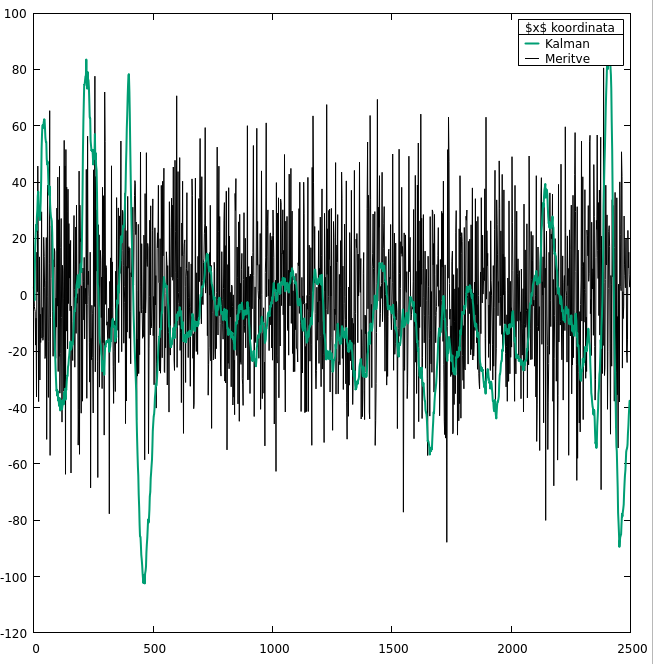
\includegraphics{graf5}}%
    \gplfronttext
  \end{picture}%
\endgroup
} 
    \resizebox{0.49\linewidth}{!}{% GNUPLOT: LaTeX picture with Postscript
\begingroup
  \makeatletter
  \providecommand\color[2][]{%
    \GenericError{(gnuplot) \space\space\space\@spaces}{%
      Package color not loaded in conjunction with
      terminal option `colourtext'%
    }{See the gnuplot documentation for explanation.%
    }{Either use 'blacktext' in gnuplot or load the package
      color.sty in LaTeX.}%
    \renewcommand\color[2][]{}%
  }%
  \providecommand\includegraphics[2][]{%
    \GenericError{(gnuplot) \space\space\space\@spaces}{%
      Package graphicx or graphics not loaded%
    }{See the gnuplot documentation for explanation.%
    }{The gnuplot epslatex terminal needs graphicx.sty or graphics.sty.}%
    \renewcommand\includegraphics[2][]{}%
  }%
  \providecommand\rotatebox[2]{#2}%
  \@ifundefined{ifGPcolor}{%
    \newif\ifGPcolor
    \GPcolortrue
  }{}%
  \@ifundefined{ifGPblacktext}{%
    \newif\ifGPblacktext
    \GPblacktexttrue
  }{}%
  % define a \g@addto@macro without @ in the name:
  \let\gplgaddtomacro\g@addto@macro
  % define empty templates for all commands taking text:
  \gdef\gplbacktext{}%
  \gdef\gplfronttext{}%
  \makeatother
  \ifGPblacktext
    % no textcolor at all
    \def\colorrgb#1{}%
    \def\colorgray#1{}%
  \else
    % gray or color?
    \ifGPcolor
      \def\colorrgb#1{\color[rgb]{#1}}%
      \def\colorgray#1{\color[gray]{#1}}%
      \expandafter\def\csname LTw\endcsname{\color{white}}%
      \expandafter\def\csname LTb\endcsname{\color{black}}%
      \expandafter\def\csname LTa\endcsname{\color{black}}%
      \expandafter\def\csname LT0\endcsname{\color[rgb]{1,0,0}}%
      \expandafter\def\csname LT1\endcsname{\color[rgb]{0,1,0}}%
      \expandafter\def\csname LT2\endcsname{\color[rgb]{0,0,1}}%
      \expandafter\def\csname LT3\endcsname{\color[rgb]{1,0,1}}%
      \expandafter\def\csname LT4\endcsname{\color[rgb]{0,1,1}}%
      \expandafter\def\csname LT5\endcsname{\color[rgb]{1,1,0}}%
      \expandafter\def\csname LT6\endcsname{\color[rgb]{0,0,0}}%
      \expandafter\def\csname LT7\endcsname{\color[rgb]{1,0.3,0}}%
      \expandafter\def\csname LT8\endcsname{\color[rgb]{0.5,0.5,0.5}}%
    \else
      % gray
      \def\colorrgb#1{\color{black}}%
      \def\colorgray#1{\color[gray]{#1}}%
      \expandafter\def\csname LTw\endcsname{\color{white}}%
      \expandafter\def\csname LTb\endcsname{\color{black}}%
      \expandafter\def\csname LTa\endcsname{\color{black}}%
      \expandafter\def\csname LT0\endcsname{\color{black}}%
      \expandafter\def\csname LT1\endcsname{\color{black}}%
      \expandafter\def\csname LT2\endcsname{\color{black}}%
      \expandafter\def\csname LT3\endcsname{\color{black}}%
      \expandafter\def\csname LT4\endcsname{\color{black}}%
      \expandafter\def\csname LT5\endcsname{\color{black}}%
      \expandafter\def\csname LT6\endcsname{\color{black}}%
      \expandafter\def\csname LT7\endcsname{\color{black}}%
      \expandafter\def\csname LT8\endcsname{\color{black}}%
    \fi
  \fi
    \setlength{\unitlength}{0.0500bp}%
    \ifx\gptboxheight\undefined%
      \newlength{\gptboxheight}%
      \newlength{\gptboxwidth}%
      \newsavebox{\gptboxtext}%
    \fi%
    \setlength{\fboxrule}{0.5pt}%
    \setlength{\fboxsep}{1pt}%
\begin{picture}(7200.00,5040.00)%
    \gplgaddtomacro\gplbacktext{%
      \csname LTb\endcsname%%
      \put(594,220){\makebox(0,0)[r]{\strut{}$-18$}}%
      \csname LTb\endcsname%%
      \put(594,950){\makebox(0,0)[r]{\strut{}$-15$}}%
      \csname LTb\endcsname%%
      \put(594,1680){\makebox(0,0)[r]{\strut{}$-12$}}%
      \csname LTb\endcsname%%
      \put(594,2410){\makebox(0,0)[r]{\strut{}$-9$}}%
      \csname LTb\endcsname%%
      \put(594,3139){\makebox(0,0)[r]{\strut{}$-6$}}%
      \csname LTb\endcsname%%
      \put(594,3869){\makebox(0,0)[r]{\strut{}$-3$}}%
      \csname LTb\endcsname%%
      \put(594,4599){\makebox(0,0)[r]{\strut{}$0$}}%
      \csname LTb\endcsname%%
      \put(726,0){\makebox(0,0){\strut{}}}%
      \csname LTb\endcsname%%
      \put(2245,0){\makebox(0,0){\strut{}}}%
      \csname LTb\endcsname%%
      \put(3765,0){\makebox(0,0){\strut{}}}%
      \csname LTb\endcsname%%
      \put(5284,0){\makebox(0,0){\strut{}}}%
      \csname LTb\endcsname%%
      \put(6803,0){\makebox(0,0){\strut{}}}%
      \put(726,4819){\makebox(0,0){\strut{}$0$}}%
      \put(2245,4819){\makebox(0,0){\strut{}$4$}}%
      \put(3765,4819){\makebox(0,0){\strut{}$8$}}%
      \put(5284,4819){\makebox(0,0){\strut{}$12$}}%
      \put(6803,4819){\makebox(0,0){\strut{}$16$}}%
    }%
    \gplgaddtomacro\gplfronttext{%
      \csname LTb\endcsname%%
      \put(3764,4426){\makebox(0,0){\strut{}poljubni}}%
      \csname LTb\endcsname%%
      \put(3334,3084){\makebox(0,0)[l]{\strut{}$T = 0 $}}%
      \csname LTb\endcsname%%
      \put(3334,3304){\makebox(0,0)[l]{\strut{}$T = 0.1 $}}%
      \csname LTb\endcsname%%
      \put(3334,3524){\makebox(0,0)[l]{\strut{}$T = 0.25 $}}%
      \csname LTb\endcsname%%
      \put(3334,3744){\makebox(0,0)[l]{\strut{}$T = 0.5 $}}%
      \csname LTb\endcsname%%
      \put(3334,3964){\makebox(0,0)[l]{\strut{}$T = 1 $}}%
      \csname LTb\endcsname%%
      \put(3334,4184){\makebox(0,0)[l]{\strut{}$T = 5 $}}%
    }%
    \gplbacktext
    \put(0,0){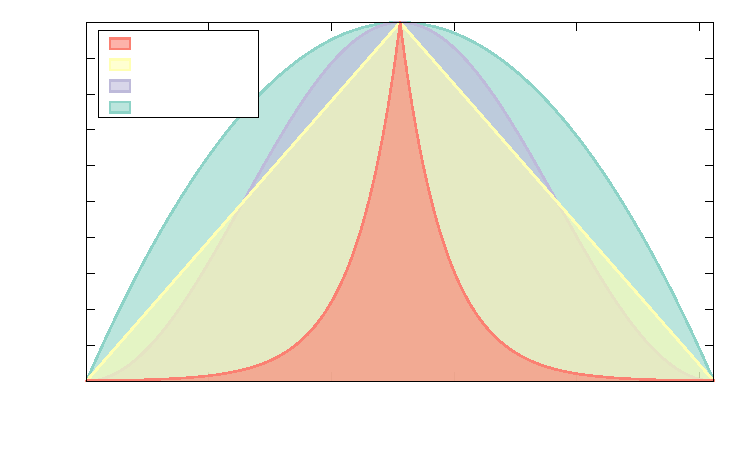
\includegraphics{graf4}}%
    \gplfronttext
  \end{picture}%
\endgroup
} 
    \resizebox{0.49\linewidth}{!}{% GNUPLOT: LaTeX picture with Postscript
\begingroup
  \makeatletter
  \providecommand\color[2][]{%
    \GenericError{(gnuplot) \space\space\space\@spaces}{%
      Package color not loaded in conjunction with
      terminal option `colourtext'%
    }{See the gnuplot documentation for explanation.%
    }{Either use 'blacktext' in gnuplot or load the package
      color.sty in LaTeX.}%
    \renewcommand\color[2][]{}%
  }%
  \providecommand\includegraphics[2][]{%
    \GenericError{(gnuplot) \space\space\space\@spaces}{%
      Package graphicx or graphics not loaded%
    }{See the gnuplot documentation for explanation.%
    }{The gnuplot epslatex terminal needs graphicx.sty or graphics.sty.}%
    \renewcommand\includegraphics[2][]{}%
  }%
  \providecommand\rotatebox[2]{#2}%
  \@ifundefined{ifGPcolor}{%
    \newif\ifGPcolor
    \GPcolortrue
  }{}%
  \@ifundefined{ifGPblacktext}{%
    \newif\ifGPblacktext
    \GPblacktexttrue
  }{}%
  % define a \g@addto@macro without @ in the name:
  \let\gplgaddtomacro\g@addto@macro
  % define empty templates for all commands taking text:
  \gdef\gplbacktext{}%
  \gdef\gplfronttext{}%
  \makeatother
  \ifGPblacktext
    % no textcolor at all
    \def\colorrgb#1{}%
    \def\colorgray#1{}%
  \else
    % gray or color?
    \ifGPcolor
      \def\colorrgb#1{\color[rgb]{#1}}%
      \def\colorgray#1{\color[gray]{#1}}%
      \expandafter\def\csname LTw\endcsname{\color{white}}%
      \expandafter\def\csname LTb\endcsname{\color{black}}%
      \expandafter\def\csname LTa\endcsname{\color{black}}%
      \expandafter\def\csname LT0\endcsname{\color[rgb]{1,0,0}}%
      \expandafter\def\csname LT1\endcsname{\color[rgb]{0,1,0}}%
      \expandafter\def\csname LT2\endcsname{\color[rgb]{0,0,1}}%
      \expandafter\def\csname LT3\endcsname{\color[rgb]{1,0,1}}%
      \expandafter\def\csname LT4\endcsname{\color[rgb]{0,1,1}}%
      \expandafter\def\csname LT5\endcsname{\color[rgb]{1,1,0}}%
      \expandafter\def\csname LT6\endcsname{\color[rgb]{0,0,0}}%
      \expandafter\def\csname LT7\endcsname{\color[rgb]{1,0.3,0}}%
      \expandafter\def\csname LT8\endcsname{\color[rgb]{0.5,0.5,0.5}}%
    \else
      % gray
      \def\colorrgb#1{\color{black}}%
      \def\colorgray#1{\color[gray]{#1}}%
      \expandafter\def\csname LTw\endcsname{\color{white}}%
      \expandafter\def\csname LTb\endcsname{\color{black}}%
      \expandafter\def\csname LTa\endcsname{\color{black}}%
      \expandafter\def\csname LT0\endcsname{\color{black}}%
      \expandafter\def\csname LT1\endcsname{\color{black}}%
      \expandafter\def\csname LT2\endcsname{\color{black}}%
      \expandafter\def\csname LT3\endcsname{\color{black}}%
      \expandafter\def\csname LT4\endcsname{\color{black}}%
      \expandafter\def\csname LT5\endcsname{\color{black}}%
      \expandafter\def\csname LT6\endcsname{\color{black}}%
      \expandafter\def\csname LT7\endcsname{\color{black}}%
      \expandafter\def\csname LT8\endcsname{\color{black}}%
    \fi
  \fi
    \setlength{\unitlength}{0.0500bp}%
    \ifx\gptboxheight\undefined%
      \newlength{\gptboxheight}%
      \newlength{\gptboxwidth}%
      \newsavebox{\gptboxtext}%
    \fi%
    \setlength{\fboxrule}{0.5pt}%
    \setlength{\fboxsep}{1pt}%
\begin{picture}(7200.00,5040.00)%
    \gplgaddtomacro\gplbacktext{%
      \csname LTb\endcsname%%
      \put(594,220){\makebox(0,0)[r]{\strut{}$-18$}}%
      \csname LTb\endcsname%%
      \put(594,950){\makebox(0,0)[r]{\strut{}$-15$}}%
      \csname LTb\endcsname%%
      \put(594,1680){\makebox(0,0)[r]{\strut{}$-12$}}%
      \csname LTb\endcsname%%
      \put(594,2410){\makebox(0,0)[r]{\strut{}$-9$}}%
      \csname LTb\endcsname%%
      \put(594,3139){\makebox(0,0)[r]{\strut{}$-6$}}%
      \csname LTb\endcsname%%
      \put(594,3869){\makebox(0,0)[r]{\strut{}$-3$}}%
      \csname LTb\endcsname%%
      \put(594,4599){\makebox(0,0)[r]{\strut{}$0$}}%
      \csname LTb\endcsname%%
      \put(726,0){\makebox(0,0){\strut{}}}%
      \csname LTb\endcsname%%
      \put(2245,0){\makebox(0,0){\strut{}}}%
      \csname LTb\endcsname%%
      \put(3765,0){\makebox(0,0){\strut{}}}%
      \csname LTb\endcsname%%
      \put(5284,0){\makebox(0,0){\strut{}}}%
      \csname LTb\endcsname%%
      \put(6803,0){\makebox(0,0){\strut{}}}%
      \put(726,4819){\makebox(0,0){\strut{}$0$}}%
      \put(2245,4819){\makebox(0,0){\strut{}$4$}}%
      \put(3765,4819){\makebox(0,0){\strut{}$8$}}%
      \put(5284,4819){\makebox(0,0){\strut{}$12$}}%
      \put(6803,4819){\makebox(0,0){\strut{}$16$}}%
    }%
    \gplgaddtomacro\gplfronttext{%
      \csname LTb\endcsname%%
      \put(3764,4426){\makebox(0,0){\strut{}zvezni nivoji}}%
      \csname LTb\endcsname%%
      \put(3299,3084){\makebox(0,0)[l]{\strut{}$$T = 0$$}}%
      \csname LTb\endcsname%%
      \put(3299,3304){\makebox(0,0)[l]{\strut{}$T = 0.1$}}%
      \csname LTb\endcsname%%
      \put(3299,3524){\makebox(0,0)[l]{\strut{}$T = 0.25 $}}%
      \csname LTb\endcsname%%
      \put(3299,3744){\makebox(0,0)[l]{\strut{}$T = 0.5 $}}%
      \csname LTb\endcsname%%
      \put(3299,3964){\makebox(0,0)[l]{\strut{}$T = 1 $}}%
      \csname LTb\endcsname%%
      \put(3299,4184){\makebox(0,0)[l]{\strut{}$T=5 $}}%
    }%
    \gplbacktext
    \put(0,0){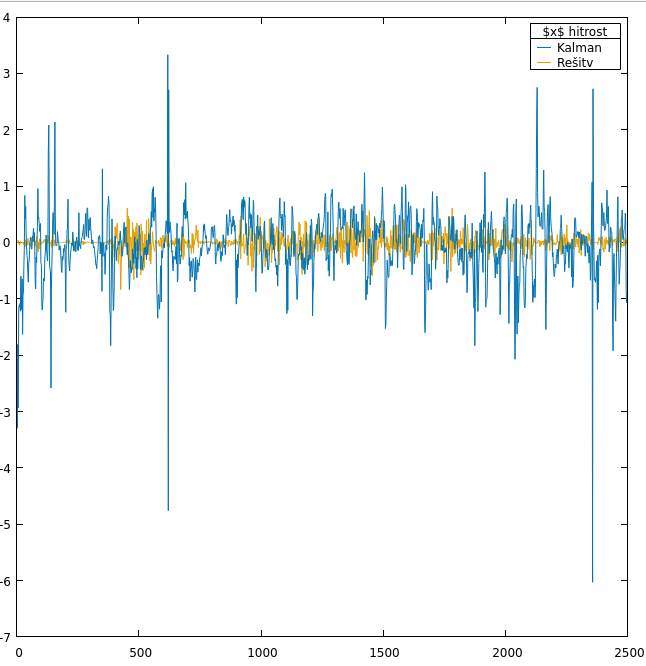
\includegraphics{graf3}}%
    \gplfronttext
  \end{picture}%
\endgroup
} 
    \caption{Primerjava spreminjanja končnega stanja z~večanjem temperature.}
    \label{slika2}
\end{figure}

Z~večanjem temperature sistemu damo možnost, da sprejme novo stanje, tudi če energijsko ni
bolj ugodno. Na grafih~\ref{slika2} so prikazana končna stanja pri različnih 
temperaturah $T$ (razmerje $k_{\text{B}} T/\Delta E$). Kot lahko predvidimo, se pri višanju 
temperature oblika sistema odmika od pričakovane za prosto visečo verižnico ($y = a \cosh 
(x/a)$). 
Obnašanje si lahko razložimo tudi s~spreminjanjem energije. Z~grafa~\ref{slika4} vidimo,
da energija že pri nekje $200$ korakih pride do končne vrednosti in potem le še niha
okoli te vrednosti. To je opazno tudi v~animaciji, ko je model že v končni vrednosti,
pa vseeno še naprej skače okoli nje, saj smo v~veliko manj korakih dosegli željeno končno
vrednost modela, kot smo imeli korakov v~algoritmu.
\begin{figure}    
    \centering 
    \resizebox{0.93\linewidth}{!}{% GNUPLOT: LaTeX picture with Postscript
\begingroup
  \makeatletter
  \providecommand\color[2][]{%
    \GenericError{(gnuplot) \space\space\space\@spaces}{%
      Package color not loaded in conjunction with
      terminal option `colourtext'%
    }{See the gnuplot documentation for explanation.%
    }{Either use 'blacktext' in gnuplot or load the package
      color.sty in LaTeX.}%
    \renewcommand\color[2][]{}%
  }%
  \providecommand\includegraphics[2][]{%
    \GenericError{(gnuplot) \space\space\space\@spaces}{%
      Package graphicx or graphics not loaded%
    }{See the gnuplot documentation for explanation.%
    }{The gnuplot epslatex terminal needs graphicx.sty or graphics.sty.}%
    \renewcommand\includegraphics[2][]{}%
  }%
  \providecommand\rotatebox[2]{#2}%
  \@ifundefined{ifGPcolor}{%
    \newif\ifGPcolor
    \GPcolortrue
  }{}%
  \@ifundefined{ifGPblacktext}{%
    \newif\ifGPblacktext
    \GPblacktexttrue
  }{}%
  % define a \g@addto@macro without @ in the name:
  \let\gplgaddtomacro\g@addto@macro
  % define empty templates for all commands taking text:
  \gdef\gplbacktext{}%
  \gdef\gplfronttext{}%
  \makeatother
  \ifGPblacktext
    % no textcolor at all
    \def\colorrgb#1{}%
    \def\colorgray#1{}%
  \else
    % gray or color?
    \ifGPcolor
      \def\colorrgb#1{\color[rgb]{#1}}%
      \def\colorgray#1{\color[gray]{#1}}%
      \expandafter\def\csname LTw\endcsname{\color{white}}%
      \expandafter\def\csname LTb\endcsname{\color{black}}%
      \expandafter\def\csname LTa\endcsname{\color{black}}%
      \expandafter\def\csname LT0\endcsname{\color[rgb]{1,0,0}}%
      \expandafter\def\csname LT1\endcsname{\color[rgb]{0,1,0}}%
      \expandafter\def\csname LT2\endcsname{\color[rgb]{0,0,1}}%
      \expandafter\def\csname LT3\endcsname{\color[rgb]{1,0,1}}%
      \expandafter\def\csname LT4\endcsname{\color[rgb]{0,1,1}}%
      \expandafter\def\csname LT5\endcsname{\color[rgb]{1,1,0}}%
      \expandafter\def\csname LT6\endcsname{\color[rgb]{0,0,0}}%
      \expandafter\def\csname LT7\endcsname{\color[rgb]{1,0.3,0}}%
      \expandafter\def\csname LT8\endcsname{\color[rgb]{0.5,0.5,0.5}}%
    \else
      % gray
      \def\colorrgb#1{\color{black}}%
      \def\colorgray#1{\color[gray]{#1}}%
      \expandafter\def\csname LTw\endcsname{\color{white}}%
      \expandafter\def\csname LTb\endcsname{\color{black}}%
      \expandafter\def\csname LTa\endcsname{\color{black}}%
      \expandafter\def\csname LT0\endcsname{\color{black}}%
      \expandafter\def\csname LT1\endcsname{\color{black}}%
      \expandafter\def\csname LT2\endcsname{\color{black}}%
      \expandafter\def\csname LT3\endcsname{\color{black}}%
      \expandafter\def\csname LT4\endcsname{\color{black}}%
      \expandafter\def\csname LT5\endcsname{\color{black}}%
      \expandafter\def\csname LT6\endcsname{\color{black}}%
      \expandafter\def\csname LT7\endcsname{\color{black}}%
      \expandafter\def\csname LT8\endcsname{\color{black}}%
    \fi
  \fi
    \setlength{\unitlength}{0.0500bp}%
    \ifx\gptboxheight\undefined%
      \newlength{\gptboxheight}%
      \newlength{\gptboxwidth}%
      \newsavebox{\gptboxtext}%
    \fi%
    \setlength{\fboxrule}{0.5pt}%
    \setlength{\fboxsep}{1pt}%
\begin{picture}(7200.00,5040.00)%
    \gplgaddtomacro\gplbacktext{%
      \csname LTb\endcsname%%
      \put(462,440){\makebox(0,0)[r]{\strut{}$0$}}%
      \put(462,1316){\makebox(0,0)[r]{\strut{}$5$}}%
      \put(462,2192){\makebox(0,0)[r]{\strut{}$10$}}%
      \put(462,3067){\makebox(0,0)[r]{\strut{}$15$}}%
      \put(462,3943){\makebox(0,0)[r]{\strut{}$20$}}%
      \put(462,4819){\makebox(0,0)[r]{\strut{}$25$}}%
      \put(594,220){\makebox(0,0){\strut{}$0$}}%
      \put(1836,220){\makebox(0,0){\strut{}$2$}}%
      \put(3078,220){\makebox(0,0){\strut{}$4$}}%
      \put(4319,220){\makebox(0,0){\strut{}$6$}}%
      \put(5561,220){\makebox(0,0){\strut{}$8$}}%
      \put(6803,220){\makebox(0,0){\strut{}$10$}}%
    }%
    \gplgaddtomacro\gplfronttext{%
      \csname LTb\endcsname%%
      \put(5086,3216){\makebox(0,0)[l]{\strut{}$ \Delta t = 0.001$}}%
      \csname LTb\endcsname%%
      \put(5086,3436){\makebox(0,0)[l]{\strut{}$ \Delta t = 0.01$}}%
      \csname LTb\endcsname%%
      \put(5086,3656){\makebox(0,0)[l]{\strut{}$ \Delta t = 0.1$}}%
      \csname LTb\endcsname%%
      \put(5086,3876){\makebox(0,0)[l]{\strut{}$ \Delta t = 0.25$}}%
      \csname LTb\endcsname%%
      \put(5086,4096){\makebox(0,0)[l]{\strut{}$ \Delta t = 0.5$}}%
      \csname LTb\endcsname%%
      \put(5086,4316){\makebox(0,0)[l]{\strut{}$ \Delta t = 1$}}%
      \csname LTb\endcsname%%
      \put(5086,4536){\makebox(0,0)[l]{\strut{}$N_0 \mathrm{e}^{-\beta t}$}}%
    }%
    \gplbacktext
    \put(0,0){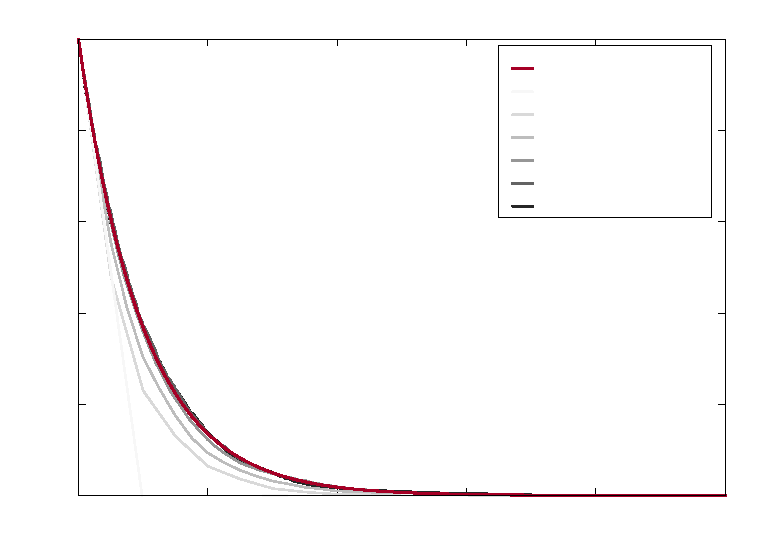
\includegraphics[width={360.00bp},height={252.00bp}]{graf6}}%
    \gplfronttext
  \end{picture}%
\endgroup
} 
    %\resizebox{0.49\linewidth}{!}{% GNUPLOT: LaTeX picture with Postscript
\begingroup
  \makeatletter
  \providecommand\color[2][]{%
    \GenericError{(gnuplot) \space\space\space\@spaces}{%
      Package color not loaded in conjunction with
      terminal option `colourtext'%
    }{See the gnuplot documentation for explanation.%
    }{Either use 'blacktext' in gnuplot or load the package
      color.sty in LaTeX.}%
    \renewcommand\color[2][]{}%
  }%
  \providecommand\includegraphics[2][]{%
    \GenericError{(gnuplot) \space\space\space\@spaces}{%
      Package graphicx or graphics not loaded%
    }{See the gnuplot documentation for explanation.%
    }{The gnuplot epslatex terminal needs graphicx.sty or graphics.sty.}%
    \renewcommand\includegraphics[2][]{}%
  }%
  \providecommand\rotatebox[2]{#2}%
  \@ifundefined{ifGPcolor}{%
    \newif\ifGPcolor
    \GPcolortrue
  }{}%
  \@ifundefined{ifGPblacktext}{%
    \newif\ifGPblacktext
    \GPblacktexttrue
  }{}%
  % define a \g@addto@macro without @ in the name:
  \let\gplgaddtomacro\g@addto@macro
  % define empty templates for all commands taking text:
  \gdef\gplbacktext{}%
  \gdef\gplfronttext{}%
  \makeatother
  \ifGPblacktext
    % no textcolor at all
    \def\colorrgb#1{}%
    \def\colorgray#1{}%
  \else
    % gray or color?
    \ifGPcolor
      \def\colorrgb#1{\color[rgb]{#1}}%
      \def\colorgray#1{\color[gray]{#1}}%
      \expandafter\def\csname LTw\endcsname{\color{white}}%
      \expandafter\def\csname LTb\endcsname{\color{black}}%
      \expandafter\def\csname LTa\endcsname{\color{black}}%
      \expandafter\def\csname LT0\endcsname{\color[rgb]{1,0,0}}%
      \expandafter\def\csname LT1\endcsname{\color[rgb]{0,1,0}}%
      \expandafter\def\csname LT2\endcsname{\color[rgb]{0,0,1}}%
      \expandafter\def\csname LT3\endcsname{\color[rgb]{1,0,1}}%
      \expandafter\def\csname LT4\endcsname{\color[rgb]{0,1,1}}%
      \expandafter\def\csname LT5\endcsname{\color[rgb]{1,1,0}}%
      \expandafter\def\csname LT6\endcsname{\color[rgb]{0,0,0}}%
      \expandafter\def\csname LT7\endcsname{\color[rgb]{1,0.3,0}}%
      \expandafter\def\csname LT8\endcsname{\color[rgb]{0.5,0.5,0.5}}%
    \else
      % gray
      \def\colorrgb#1{\color{black}}%
      \def\colorgray#1{\color[gray]{#1}}%
      \expandafter\def\csname LTw\endcsname{\color{white}}%
      \expandafter\def\csname LTb\endcsname{\color{black}}%
      \expandafter\def\csname LTa\endcsname{\color{black}}%
      \expandafter\def\csname LT0\endcsname{\color{black}}%
      \expandafter\def\csname LT1\endcsname{\color{black}}%
      \expandafter\def\csname LT2\endcsname{\color{black}}%
      \expandafter\def\csname LT3\endcsname{\color{black}}%
      \expandafter\def\csname LT4\endcsname{\color{black}}%
      \expandafter\def\csname LT5\endcsname{\color{black}}%
      \expandafter\def\csname LT6\endcsname{\color{black}}%
      \expandafter\def\csname LT7\endcsname{\color{black}}%
      \expandafter\def\csname LT8\endcsname{\color{black}}%
    \fi
  \fi
    \setlength{\unitlength}{0.0500bp}%
    \ifx\gptboxheight\undefined%
      \newlength{\gptboxheight}%
      \newlength{\gptboxwidth}%
      \newsavebox{\gptboxtext}%
    \fi%
    \setlength{\fboxrule}{0.5pt}%
    \setlength{\fboxsep}{1pt}%
\begin{picture}(7200.00,5040.00)%
    \gplgaddtomacro\gplbacktext{%
      \csname LTb\endcsname%%
      \put(594,440){\makebox(0,0)[r]{\strut{}$0.1$}}%
      \put(594,1900){\makebox(0,0)[r]{\strut{}$1$}}%
      \put(594,3359){\makebox(0,0)[r]{\strut{}$10$}}%
      \put(594,4819){\makebox(0,0)[r]{\strut{}$100$}}%
      \put(726,220){\makebox(0,0){\strut{}$0$}}%
      \put(1941,220){\makebox(0,0){\strut{}$2$}}%
      \put(3157,220){\makebox(0,0){\strut{}$4$}}%
      \put(4372,220){\makebox(0,0){\strut{}$6$}}%
      \put(5588,220){\makebox(0,0){\strut{}$8$}}%
      \put(6803,220){\makebox(0,0){\strut{}$10$}}%
    }%
    \gplgaddtomacro\gplfronttext{%
      \csname LTb\endcsname%%
      \put(5086,3216){\makebox(0,0)[l]{\strut{}$ \Delta t = 0.001$}}%
      \csname LTb\endcsname%%
      \put(5086,3436){\makebox(0,0)[l]{\strut{}$ \Delta t = 0.01$}}%
      \csname LTb\endcsname%%
      \put(5086,3656){\makebox(0,0)[l]{\strut{}$ \Delta t = 0.1$}}%
      \csname LTb\endcsname%%
      \put(5086,3876){\makebox(0,0)[l]{\strut{}$ \Delta t = 0.25$}}%
      \csname LTb\endcsname%%
      \put(5086,4096){\makebox(0,0)[l]{\strut{}$ \Delta t = 0.5$}}%
      \csname LTb\endcsname%%
      \put(5086,4316){\makebox(0,0)[l]{\strut{}$ \Delta t = 1$}}%
      \csname LTb\endcsname%%
      \put(5086,4536){\makebox(0,0)[l]{\strut{}$N_0 \mathrm{e}^{-\beta t}$}}%
    }%
    \gplbacktext
    \put(0,0){\includegraphics[width={360.00bp},height={252.00bp}]{graf7}}%
    \gplfronttext
  \end{picture}%
\endgroup
} 
    \caption{Spreminjanje energije pri temperaturi $T=0$} 
    \label{slika4}
\end{figure}


\pagebreak

%----------------------------------------------------------------------------------------
%	PROBLEM 2
%----------------------------------------------------------------------------------------
\section{Isingov model}
S~Hamiltonijanom
\begin{equation}
    \mathcal{H} = -J \sum_{\evdel{i,j}}s_i s_j - H \sum_i s_i, \quad J=\pm 1
\end{equation}
opišemo feromagnetne ($J=1$) in antiferomagnetne ($J=-1$) snovi. Približek velja za dve 
stanji $s_i = \pm 1$, vsota $\sum_{\evdel{ij}}$ pa teče po vezeh med najbližjimi sosedi. 
Če ni zunanjega polja $H=0$, temperatura $T_{\text{c}}$ faznega prehoda pri feromagnetu 
zadošča enačbi 
\begin{equation}
    \sinh \frac{2J}{k_{\text{B}} T_{\text{c}}} = 1 \quad \Longrightarrow \quad
    T_c \approx 2.269185 \frac{J}{k_{\text{B}}}.
\end{equation}
Zanima nas povprečna energija $\evdel{E}$ in lastna magnetizacija $\evdel{S}$ v~odvisnosti
od temperature. $S = \sum_i^N s_i$ je celotna magnetizacija sistema. Zanima nas tudi 
spinska susceptibilnost in specifična toplota pri različnih jakostih magnetnega polja
\begin{equation}
    \chi = \frac{ \evdel{S^2} - \evdel{S}^2}{N k_{\text{B}} T} \qquad
    c = \frac{ \evdel{E^2} - \evdel{E}^2}{N k_{\text{B}} T}.
\end{equation}
Rešujemo podobno kot pri prejšnji nalogi; mrežo razdelimo na $N_x$ elementov v~eni smeri
in $N_y$ v~drugi, kjer vsakemu spinu pripada točka $(i,j)$. Na vsakem koraku naključno
izberemo par $i,j$, spremenimo vrednost in pogledamo kako ta sprememba vpliva na energijo 
sistema:
\begin{equation}
    \Delta E = 2 s_i \left( J \sum_{\evdel{i,j}} s_j + H \right).
\end{equation}

\subsection{Rezultati}
Poglejmo si kako se obnaša sistem brez zunanjega polja pri različnih temperaturah. Končna
stanja feromagneta so prikazana na grafih~\ref{slika3}. Vidimo, da se pri nizki 
temperaturi ustvarijo domene in imamo spontano magnetizacijo. Z~naraščanjem temperature 
se domene začnejo manjšati in premikati, spini znotraj nje pa obračati. Pri temperaturi 
$T = T_c$ (med tretjo in četrto sliko) se zgodi fazni prehod in po tem so spinska stanja 
naključna in magnetizacija pade na $0$. \\
Podobno lahko tudi pri antiferomagnetu na grafu~\ref{slika5} opazimo domene, ki so sicer 
slabše vidne, vendar se obnašajo enako kot pri feromagnetu in tudi na enak način izginejo.
Hlajenje antiferomagneta je prikazano v~animaciji \path{antiferomagnet.gif}, feromagneta pa
\path{feromagnet.gif}.\\
\begin{figure}[H]
    \centering 
    \resizebox{0.32\textwidth}{!}{% GNUPLOT: LaTeX picture with Postscript
\begingroup
  \makeatletter
  \providecommand\color[2][]{%
    \GenericError{(gnuplot) \space\space\space\@spaces}{%
      Package color not loaded in conjunction with
      terminal option `colourtext'%
    }{See the gnuplot documentation for explanation.%
    }{Either use 'blacktext' in gnuplot or load the package
      color.sty in LaTeX.}%
    \renewcommand\color[2][]{}%
  }%
  \providecommand\includegraphics[2][]{%
    \GenericError{(gnuplot) \space\space\space\@spaces}{%
      Package graphicx or graphics not loaded%
    }{See the gnuplot documentation for explanation.%
    }{The gnuplot epslatex terminal needs graphicx.sty or graphics.sty.}%
    \renewcommand\includegraphics[2][]{}%
  }%
  \providecommand\rotatebox[2]{#2}%
  \@ifundefined{ifGPcolor}{%
    \newif\ifGPcolor
    \GPcolortrue
  }{}%
  \@ifundefined{ifGPblacktext}{%
    \newif\ifGPblacktext
    \GPblacktexttrue
  }{}%
  % define a \g@addto@macro without @ in the name:
  \let\gplgaddtomacro\g@addto@macro
  % define empty templates for all commands taking text:
  \gdef\gplbacktext{}%
  \gdef\gplfronttext{}%
  \makeatother
  \ifGPblacktext
    % no textcolor at all
    \def\colorrgb#1{}%
    \def\colorgray#1{}%
  \else
    % gray or color?
    \ifGPcolor
      \def\colorrgb#1{\color[rgb]{#1}}%
      \def\colorgray#1{\color[gray]{#1}}%
      \expandafter\def\csname LTw\endcsname{\color{white}}%
      \expandafter\def\csname LTb\endcsname{\color{black}}%
      \expandafter\def\csname LTa\endcsname{\color{black}}%
      \expandafter\def\csname LT0\endcsname{\color[rgb]{1,0,0}}%
      \expandafter\def\csname LT1\endcsname{\color[rgb]{0,1,0}}%
      \expandafter\def\csname LT2\endcsname{\color[rgb]{0,0,1}}%
      \expandafter\def\csname LT3\endcsname{\color[rgb]{1,0,1}}%
      \expandafter\def\csname LT4\endcsname{\color[rgb]{0,1,1}}%
      \expandafter\def\csname LT5\endcsname{\color[rgb]{1,1,0}}%
      \expandafter\def\csname LT6\endcsname{\color[rgb]{0,0,0}}%
      \expandafter\def\csname LT7\endcsname{\color[rgb]{1,0.3,0}}%
      \expandafter\def\csname LT8\endcsname{\color[rgb]{0.5,0.5,0.5}}%
    \else
      % gray
      \def\colorrgb#1{\color{black}}%
      \def\colorgray#1{\color[gray]{#1}}%
      \expandafter\def\csname LTw\endcsname{\color{white}}%
      \expandafter\def\csname LTb\endcsname{\color{black}}%
      \expandafter\def\csname LTa\endcsname{\color{black}}%
      \expandafter\def\csname LT0\endcsname{\color{black}}%
      \expandafter\def\csname LT1\endcsname{\color{black}}%
      \expandafter\def\csname LT2\endcsname{\color{black}}%
      \expandafter\def\csname LT3\endcsname{\color{black}}%
      \expandafter\def\csname LT4\endcsname{\color{black}}%
      \expandafter\def\csname LT5\endcsname{\color{black}}%
      \expandafter\def\csname LT6\endcsname{\color{black}}%
      \expandafter\def\csname LT7\endcsname{\color{black}}%
      \expandafter\def\csname LT8\endcsname{\color{black}}%
    \fi
  \fi
    \setlength{\unitlength}{0.0500bp}%
    \ifx\gptboxheight\undefined%
      \newlength{\gptboxheight}%
      \newlength{\gptboxwidth}%
      \newsavebox{\gptboxtext}%
    \fi%
    \setlength{\fboxrule}{0.5pt}%
    \setlength{\fboxsep}{1pt}%
\begin{picture}(7200.00,5040.00)%
    \gplgaddtomacro\gplbacktext{%
      \csname LTb\endcsname%%
      \put(682,704){\makebox(0,0)[r]{\strut{}$-3$}}%
      \put(682,1292){\makebox(0,0)[r]{\strut{}$-2$}}%
      \put(682,1880){\makebox(0,0)[r]{\strut{}$-1$}}%
      \put(682,2468){\makebox(0,0)[r]{\strut{}$0$}}%
      \put(682,3055){\makebox(0,0)[r]{\strut{}$1$}}%
      \put(682,3643){\makebox(0,0)[r]{\strut{}$2$}}%
      \put(682,4231){\makebox(0,0)[r]{\strut{}$3$}}%
      \put(682,4819){\makebox(0,0)[r]{\strut{}$4$}}%
      \put(814,484){\makebox(0,0){\strut{}$0$}}%
      \put(1984,484){\makebox(0,0){\strut{}$100$}}%
      \put(3153,484){\makebox(0,0){\strut{}$200$}}%
      \put(4323,484){\makebox(0,0){\strut{}$300$}}%
      \put(5493,484){\makebox(0,0){\strut{}$400$}}%
      \put(6663,484){\makebox(0,0){\strut{}$500$}}%
    }%
    \gplgaddtomacro\gplfronttext{%
      \csname LTb\endcsname%%
      \put(209,2761){\rotatebox{-270}{\makebox(0,0){\strut{}$u_i(t)$}}}%
      \put(3808,154){\makebox(0,0){\strut{}$t$}}%
      \csname LTb\endcsname%%
      \put(5879,3986){\makebox(0,0)[l]{\strut{}signal3}}%
      \csname LTb\endcsname%%
      \put(5879,4206){\makebox(0,0)[l]{\strut{}signal2}}%
      \csname LTb\endcsname%%
      \put(5879,4426){\makebox(0,0)[l]{\strut{}signal1}}%
      \csname LTb\endcsname%%
      \put(5879,4646){\makebox(0,0)[l]{\strut{}signal0}}%
    }%
    \gplbacktext
    \put(0,0){\includegraphics[width={360.00bp},height={252.00bp}]{graf9}}%
    \gplfronttext
  \end{picture}%
\endgroup
} 
    \resizebox{0.32\textwidth}{!}{% GNUPLOT: LaTeX picture with Postscript
\begingroup
  \makeatletter
  \providecommand\color[2][]{%
    \GenericError{(gnuplot) \space\space\space\@spaces}{%
      Package color not loaded in conjunction with
      terminal option `colourtext'%
    }{See the gnuplot documentation for explanation.%
    }{Either use 'blacktext' in gnuplot or load the package
      color.sty in LaTeX.}%
    \renewcommand\color[2][]{}%
  }%
  \providecommand\includegraphics[2][]{%
    \GenericError{(gnuplot) \space\space\space\@spaces}{%
      Package graphicx or graphics not loaded%
    }{See the gnuplot documentation for explanation.%
    }{The gnuplot epslatex terminal needs graphicx.sty or graphics.sty.}%
    \renewcommand\includegraphics[2][]{}%
  }%
  \providecommand\rotatebox[2]{#2}%
  \@ifundefined{ifGPcolor}{%
    \newif\ifGPcolor
    \GPcolortrue
  }{}%
  \@ifundefined{ifGPblacktext}{%
    \newif\ifGPblacktext
    \GPblacktexttrue
  }{}%
  % define a \g@addto@macro without @ in the name:
  \let\gplgaddtomacro\g@addto@macro
  % define empty templates for all commands taking text:
  \gdef\gplbacktext{}%
  \gdef\gplfronttext{}%
  \makeatother
  \ifGPblacktext
    % no textcolor at all
    \def\colorrgb#1{}%
    \def\colorgray#1{}%
  \else
    % gray or color?
    \ifGPcolor
      \def\colorrgb#1{\color[rgb]{#1}}%
      \def\colorgray#1{\color[gray]{#1}}%
      \expandafter\def\csname LTw\endcsname{\color{white}}%
      \expandafter\def\csname LTb\endcsname{\color{black}}%
      \expandafter\def\csname LTa\endcsname{\color{black}}%
      \expandafter\def\csname LT0\endcsname{\color[rgb]{1,0,0}}%
      \expandafter\def\csname LT1\endcsname{\color[rgb]{0,1,0}}%
      \expandafter\def\csname LT2\endcsname{\color[rgb]{0,0,1}}%
      \expandafter\def\csname LT3\endcsname{\color[rgb]{1,0,1}}%
      \expandafter\def\csname LT4\endcsname{\color[rgb]{0,1,1}}%
      \expandafter\def\csname LT5\endcsname{\color[rgb]{1,1,0}}%
      \expandafter\def\csname LT6\endcsname{\color[rgb]{0,0,0}}%
      \expandafter\def\csname LT7\endcsname{\color[rgb]{1,0.3,0}}%
      \expandafter\def\csname LT8\endcsname{\color[rgb]{0.5,0.5,0.5}}%
    \else
      % gray
      \def\colorrgb#1{\color{black}}%
      \def\colorgray#1{\color[gray]{#1}}%
      \expandafter\def\csname LTw\endcsname{\color{white}}%
      \expandafter\def\csname LTb\endcsname{\color{black}}%
      \expandafter\def\csname LTa\endcsname{\color{black}}%
      \expandafter\def\csname LT0\endcsname{\color{black}}%
      \expandafter\def\csname LT1\endcsname{\color{black}}%
      \expandafter\def\csname LT2\endcsname{\color{black}}%
      \expandafter\def\csname LT3\endcsname{\color{black}}%
      \expandafter\def\csname LT4\endcsname{\color{black}}%
      \expandafter\def\csname LT5\endcsname{\color{black}}%
      \expandafter\def\csname LT6\endcsname{\color{black}}%
      \expandafter\def\csname LT7\endcsname{\color{black}}%
      \expandafter\def\csname LT8\endcsname{\color{black}}%
    \fi
  \fi
    \setlength{\unitlength}{0.0500bp}%
    \ifx\gptboxheight\undefined%
      \newlength{\gptboxheight}%
      \newlength{\gptboxwidth}%
      \newsavebox{\gptboxtext}%
    \fi%
    \setlength{\fboxrule}{0.5pt}%
    \setlength{\fboxsep}{1pt}%
\begin{picture}(11338.00,10204.00)%
    \gplgaddtomacro\gplbacktext{%
    }%
    \gplgaddtomacro\gplfronttext{%
      \csname LTb\endcsname%%
      \put(5635,9873){\makebox(0,0){\Huge $T=1.5$}}%
    }%
    \gplbacktext
    \put(0,0){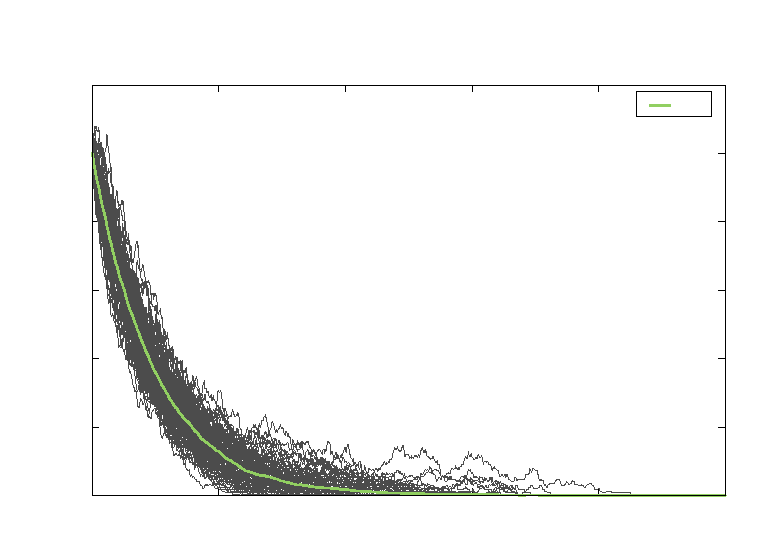
\includegraphics{graf12}}%
    \gplfronttext
  \end{picture}%
\endgroup
} 
    \resizebox{0.32\textwidth}{!}{% GNUPLOT: LaTeX picture with Postscript
\begingroup
  \makeatletter
  \providecommand\color[2][]{%
    \GenericError{(gnuplot) \space\space\space\@spaces}{%
      Package color not loaded in conjunction with
      terminal option `colourtext'%
    }{See the gnuplot documentation for explanation.%
    }{Either use 'blacktext' in gnuplot or load the package
      color.sty in LaTeX.}%
    \renewcommand\color[2][]{}%
  }%
  \providecommand\includegraphics[2][]{%
    \GenericError{(gnuplot) \space\space\space\@spaces}{%
      Package graphicx or graphics not loaded%
    }{See the gnuplot documentation for explanation.%
    }{The gnuplot epslatex terminal needs graphicx.sty or graphics.sty.}%
    \renewcommand\includegraphics[2][]{}%
  }%
  \providecommand\rotatebox[2]{#2}%
  \@ifundefined{ifGPcolor}{%
    \newif\ifGPcolor
    \GPcolortrue
  }{}%
  \@ifundefined{ifGPblacktext}{%
    \newif\ifGPblacktext
    \GPblacktexttrue
  }{}%
  % define a \g@addto@macro without @ in the name:
  \let\gplgaddtomacro\g@addto@macro
  % define empty templates for all commands taking text:
  \gdef\gplbacktext{}%
  \gdef\gplfronttext{}%
  \makeatother
  \ifGPblacktext
    % no textcolor at all
    \def\colorrgb#1{}%
    \def\colorgray#1{}%
  \else
    % gray or color?
    \ifGPcolor
      \def\colorrgb#1{\color[rgb]{#1}}%
      \def\colorgray#1{\color[gray]{#1}}%
      \expandafter\def\csname LTw\endcsname{\color{white}}%
      \expandafter\def\csname LTb\endcsname{\color{black}}%
      \expandafter\def\csname LTa\endcsname{\color{black}}%
      \expandafter\def\csname LT0\endcsname{\color[rgb]{1,0,0}}%
      \expandafter\def\csname LT1\endcsname{\color[rgb]{0,1,0}}%
      \expandafter\def\csname LT2\endcsname{\color[rgb]{0,0,1}}%
      \expandafter\def\csname LT3\endcsname{\color[rgb]{1,0,1}}%
      \expandafter\def\csname LT4\endcsname{\color[rgb]{0,1,1}}%
      \expandafter\def\csname LT5\endcsname{\color[rgb]{1,1,0}}%
      \expandafter\def\csname LT6\endcsname{\color[rgb]{0,0,0}}%
      \expandafter\def\csname LT7\endcsname{\color[rgb]{1,0.3,0}}%
      \expandafter\def\csname LT8\endcsname{\color[rgb]{0.5,0.5,0.5}}%
    \else
      % gray
      \def\colorrgb#1{\color{black}}%
      \def\colorgray#1{\color[gray]{#1}}%
      \expandafter\def\csname LTw\endcsname{\color{white}}%
      \expandafter\def\csname LTb\endcsname{\color{black}}%
      \expandafter\def\csname LTa\endcsname{\color{black}}%
      \expandafter\def\csname LT0\endcsname{\color{black}}%
      \expandafter\def\csname LT1\endcsname{\color{black}}%
      \expandafter\def\csname LT2\endcsname{\color{black}}%
      \expandafter\def\csname LT3\endcsname{\color{black}}%
      \expandafter\def\csname LT4\endcsname{\color{black}}%
      \expandafter\def\csname LT5\endcsname{\color{black}}%
      \expandafter\def\csname LT6\endcsname{\color{black}}%
      \expandafter\def\csname LT7\endcsname{\color{black}}%
      \expandafter\def\csname LT8\endcsname{\color{black}}%
    \fi
  \fi
    \setlength{\unitlength}{0.0500bp}%
    \ifx\gptboxheight\undefined%
      \newlength{\gptboxheight}%
      \newlength{\gptboxwidth}%
      \newsavebox{\gptboxtext}%
    \fi%
    \setlength{\fboxrule}{0.5pt}%
    \setlength{\fboxsep}{1pt}%
\begin{picture}(7200.00,5040.00)%
    \gplgaddtomacro\gplbacktext{%
      \csname LTb\endcsname%%
      \put(1210,704){\makebox(0,0)[r]{\strut{}$-0.004$}}%
      \put(1210,1161){\makebox(0,0)[r]{\strut{}$-0.002$}}%
      \put(1210,1618){\makebox(0,0)[r]{\strut{}$0$}}%
      \put(1210,2076){\makebox(0,0)[r]{\strut{}$0.002$}}%
      \put(1210,2533){\makebox(0,0)[r]{\strut{}$0.004$}}%
      \put(1210,2990){\makebox(0,0)[r]{\strut{}$0.006$}}%
      \put(1210,3447){\makebox(0,0)[r]{\strut{}$0.008$}}%
      \put(1210,3905){\makebox(0,0)[r]{\strut{}$0.01$}}%
      \put(1210,4362){\makebox(0,0)[r]{\strut{}$0.012$}}%
      \put(1210,4819){\makebox(0,0)[r]{\strut{}$0.014$}}%
      \put(1342,484){\makebox(0,0){\strut{}$0$}}%
      \put(2409,484){\makebox(0,0){\strut{}$100$}}%
      \put(3475,484){\makebox(0,0){\strut{}$200$}}%
      \put(4542,484){\makebox(0,0){\strut{}$300$}}%
      \put(5608,484){\makebox(0,0){\strut{}$400$}}%
      \put(6675,484){\makebox(0,0){\strut{}$500$}}%
    }%
    \gplgaddtomacro\gplfronttext{%
      \csname LTb\endcsname%%
      \put(209,2761){\rotatebox{-270}{\makebox(0,0){\strut{}$u_1(t)$}}}%
      \put(4072,154){\makebox(0,0){\strut{}$t$}}%
      \csname LTb\endcsname%%
      \put(5879,3986){\makebox(0,0)[l]{\strut{}$m=100$}}%
      \csname LTb\endcsname%%
      \put(5879,4206){\makebox(0,0)[l]{\strut{}$m=50$}}%
      \csname LTb\endcsname%%
      \put(5879,4426){\makebox(0,0)[l]{\strut{}$m=25$}}%
      \csname LTb\endcsname%%
      \put(5879,4646){\makebox(0,0)[l]{\strut{}$m=16$}}%
    }%
    \gplbacktext
    \put(0,0){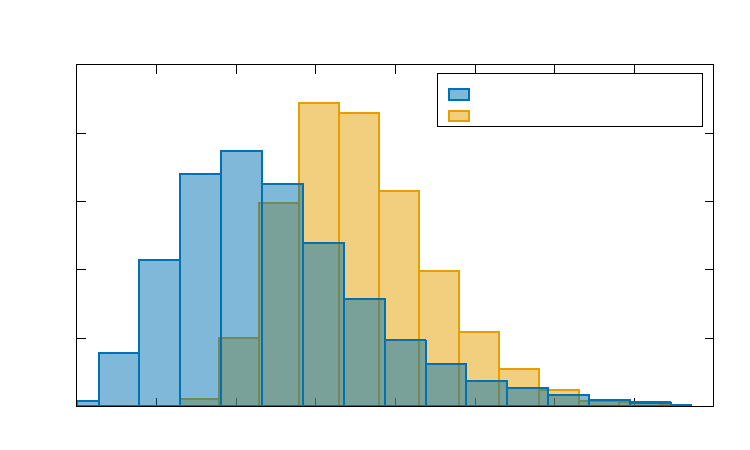
\includegraphics[width={360.00bp},height={252.00bp}]{graf13}}%
    \gplfronttext
  \end{picture}%
\endgroup
} 
    
    \resizebox{0.32\textwidth}{!}{% GNUPLOT: LaTeX picture with Postscript
\begingroup
  \makeatletter
  \providecommand\color[2][]{%
    \GenericError{(gnuplot) \space\space\space\@spaces}{%
      Package color not loaded in conjunction with
      terminal option `colourtext'%
    }{See the gnuplot documentation for explanation.%
    }{Either use 'blacktext' in gnuplot or load the package
      color.sty in LaTeX.}%
    \renewcommand\color[2][]{}%
  }%
  \providecommand\includegraphics[2][]{%
    \GenericError{(gnuplot) \space\space\space\@spaces}{%
      Package graphicx or graphics not loaded%
    }{See the gnuplot documentation for explanation.%
    }{The gnuplot epslatex terminal needs graphicx.sty or graphics.sty.}%
    \renewcommand\includegraphics[2][]{}%
  }%
  \providecommand\rotatebox[2]{#2}%
  \@ifundefined{ifGPcolor}{%
    \newif\ifGPcolor
    \GPcolortrue
  }{}%
  \@ifundefined{ifGPblacktext}{%
    \newif\ifGPblacktext
    \GPblacktexttrue
  }{}%
  % define a \g@addto@macro without @ in the name:
  \let\gplgaddtomacro\g@addto@macro
  % define empty templates for all commands taking text:
  \gdef\gplbacktext{}%
  \gdef\gplfronttext{}%
  \makeatother
  \ifGPblacktext
    % no textcolor at all
    \def\colorrgb#1{}%
    \def\colorgray#1{}%
  \else
    % gray or color?
    \ifGPcolor
      \def\colorrgb#1{\color[rgb]{#1}}%
      \def\colorgray#1{\color[gray]{#1}}%
      \expandafter\def\csname LTw\endcsname{\color{white}}%
      \expandafter\def\csname LTb\endcsname{\color{black}}%
      \expandafter\def\csname LTa\endcsname{\color{black}}%
      \expandafter\def\csname LT0\endcsname{\color[rgb]{1,0,0}}%
      \expandafter\def\csname LT1\endcsname{\color[rgb]{0,1,0}}%
      \expandafter\def\csname LT2\endcsname{\color[rgb]{0,0,1}}%
      \expandafter\def\csname LT3\endcsname{\color[rgb]{1,0,1}}%
      \expandafter\def\csname LT4\endcsname{\color[rgb]{0,1,1}}%
      \expandafter\def\csname LT5\endcsname{\color[rgb]{1,1,0}}%
      \expandafter\def\csname LT6\endcsname{\color[rgb]{0,0,0}}%
      \expandafter\def\csname LT7\endcsname{\color[rgb]{1,0.3,0}}%
      \expandafter\def\csname LT8\endcsname{\color[rgb]{0.5,0.5,0.5}}%
    \else
      % gray
      \def\colorrgb#1{\color{black}}%
      \def\colorgray#1{\color[gray]{#1}}%
      \expandafter\def\csname LTw\endcsname{\color{white}}%
      \expandafter\def\csname LTb\endcsname{\color{black}}%
      \expandafter\def\csname LTa\endcsname{\color{black}}%
      \expandafter\def\csname LT0\endcsname{\color{black}}%
      \expandafter\def\csname LT1\endcsname{\color{black}}%
      \expandafter\def\csname LT2\endcsname{\color{black}}%
      \expandafter\def\csname LT3\endcsname{\color{black}}%
      \expandafter\def\csname LT4\endcsname{\color{black}}%
      \expandafter\def\csname LT5\endcsname{\color{black}}%
      \expandafter\def\csname LT6\endcsname{\color{black}}%
      \expandafter\def\csname LT7\endcsname{\color{black}}%
      \expandafter\def\csname LT8\endcsname{\color{black}}%
    \fi
  \fi
    \setlength{\unitlength}{0.0500bp}%
    \ifx\gptboxheight\undefined%
      \newlength{\gptboxheight}%
      \newlength{\gptboxwidth}%
      \newsavebox{\gptboxtext}%
    \fi%
    \setlength{\fboxrule}{0.5pt}%
    \setlength{\fboxsep}{1pt}%
\begin{picture}(7200.00,4320.00)%
    \gplgaddtomacro\gplbacktext{%
      \csname LTb\endcsname%%
      \put(616,408){\makebox(0,0)[r]{\strut{}$0$}}%
      \csname LTb\endcsname%%
      \put(616,1064){\makebox(0,0)[r]{\strut{}$0.05$}}%
      \csname LTb\endcsname%%
      \put(616,1720){\makebox(0,0)[r]{\strut{}$0.1$}}%
      \csname LTb\endcsname%%
      \put(616,2375){\makebox(0,0)[r]{\strut{}$0.15$}}%
      \csname LTb\endcsname%%
      \put(616,3031){\makebox(0,0)[r]{\strut{}$0.2$}}%
      \csname LTb\endcsname%%
      \put(616,3687){\makebox(0,0)[r]{\strut{}$0.25$}}%
      \csname LTb\endcsname%%
      \put(728,204){\makebox(0,0){\strut{}$2$}}%
      \csname LTb\endcsname%%
      \put(1492,204){\makebox(0,0){\strut{}$3$}}%
      \csname LTb\endcsname%%
      \put(2257,204){\makebox(0,0){\strut{}$4$}}%
      \csname LTb\endcsname%%
      \put(3021,204){\makebox(0,0){\strut{}$5$}}%
      \csname LTb\endcsname%%
      \put(3786,204){\makebox(0,0){\strut{}$6$}}%
      \csname LTb\endcsname%%
      \put(4550,204){\makebox(0,0){\strut{}$7$}}%
      \csname LTb\endcsname%%
      \put(5314,204){\makebox(0,0){\strut{}$8$}}%
      \csname LTb\endcsname%%
      \put(6079,204){\makebox(0,0){\strut{}$9$}}%
      \csname LTb\endcsname%%
      \put(6843,204){\makebox(0,0){\strut{}$10$}}%
    }%
    \gplgaddtomacro\gplfronttext{%
      \csname LTb\endcsname%%
      \put(4603,3198){\makebox(0,0)[l]{\strut{}$\beta =1$}}%
      \csname LTb\endcsname%%
      \put(4603,3402){\makebox(0,0)[l]{\strut{}$\beta_s =5 \beta, \, \beta_r=4\beta$}}%
      \csname LTb\endcsname%%
      \put(3785,3993){\makebox(0,0){\strut{}$N_0=250$}}%
    }%
    \gplbacktext
    \put(0,0){\includegraphics[width={360.00bp},height={216.00bp}]{graf14}}%
    \gplfronttext
  \end{picture}%
\endgroup
} 
    \resizebox{0.32\textwidth}{!}{% GNUPLOT: LaTeX picture with Postscript
\begingroup
  \makeatletter
  \providecommand\color[2][]{%
    \GenericError{(gnuplot) \space\space\space\@spaces}{%
      Package color not loaded in conjunction with
      terminal option `colourtext'%
    }{See the gnuplot documentation for explanation.%
    }{Either use 'blacktext' in gnuplot or load the package
      color.sty in LaTeX.}%
    \renewcommand\color[2][]{}%
  }%
  \providecommand\includegraphics[2][]{%
    \GenericError{(gnuplot) \space\space\space\@spaces}{%
      Package graphicx or graphics not loaded%
    }{See the gnuplot documentation for explanation.%
    }{The gnuplot epslatex terminal needs graphicx.sty or graphics.sty.}%
    \renewcommand\includegraphics[2][]{}%
  }%
  \providecommand\rotatebox[2]{#2}%
  \@ifundefined{ifGPcolor}{%
    \newif\ifGPcolor
    \GPcolortrue
  }{}%
  \@ifundefined{ifGPblacktext}{%
    \newif\ifGPblacktext
    \GPblacktexttrue
  }{}%
  % define a \g@addto@macro without @ in the name:
  \let\gplgaddtomacro\g@addto@macro
  % define empty templates for all commands taking text:
  \gdef\gplbacktext{}%
  \gdef\gplfronttext{}%
  \makeatother
  \ifGPblacktext
    % no textcolor at all
    \def\colorrgb#1{}%
    \def\colorgray#1{}%
  \else
    % gray or color?
    \ifGPcolor
      \def\colorrgb#1{\color[rgb]{#1}}%
      \def\colorgray#1{\color[gray]{#1}}%
      \expandafter\def\csname LTw\endcsname{\color{white}}%
      \expandafter\def\csname LTb\endcsname{\color{black}}%
      \expandafter\def\csname LTa\endcsname{\color{black}}%
      \expandafter\def\csname LT0\endcsname{\color[rgb]{1,0,0}}%
      \expandafter\def\csname LT1\endcsname{\color[rgb]{0,1,0}}%
      \expandafter\def\csname LT2\endcsname{\color[rgb]{0,0,1}}%
      \expandafter\def\csname LT3\endcsname{\color[rgb]{1,0,1}}%
      \expandafter\def\csname LT4\endcsname{\color[rgb]{0,1,1}}%
      \expandafter\def\csname LT5\endcsname{\color[rgb]{1,1,0}}%
      \expandafter\def\csname LT6\endcsname{\color[rgb]{0,0,0}}%
      \expandafter\def\csname LT7\endcsname{\color[rgb]{1,0.3,0}}%
      \expandafter\def\csname LT8\endcsname{\color[rgb]{0.5,0.5,0.5}}%
    \else
      % gray
      \def\colorrgb#1{\color{black}}%
      \def\colorgray#1{\color[gray]{#1}}%
      \expandafter\def\csname LTw\endcsname{\color{white}}%
      \expandafter\def\csname LTb\endcsname{\color{black}}%
      \expandafter\def\csname LTa\endcsname{\color{black}}%
      \expandafter\def\csname LT0\endcsname{\color{black}}%
      \expandafter\def\csname LT1\endcsname{\color{black}}%
      \expandafter\def\csname LT2\endcsname{\color{black}}%
      \expandafter\def\csname LT3\endcsname{\color{black}}%
      \expandafter\def\csname LT4\endcsname{\color{black}}%
      \expandafter\def\csname LT5\endcsname{\color{black}}%
      \expandafter\def\csname LT6\endcsname{\color{black}}%
      \expandafter\def\csname LT7\endcsname{\color{black}}%
      \expandafter\def\csname LT8\endcsname{\color{black}}%
    \fi
  \fi
    \setlength{\unitlength}{0.0500bp}%
    \ifx\gptboxheight\undefined%
      \newlength{\gptboxheight}%
      \newlength{\gptboxwidth}%
      \newsavebox{\gptboxtext}%
    \fi%
    \setlength{\fboxrule}{0.5pt}%
    \setlength{\fboxsep}{1pt}%
\begin{picture}(11338.00,10204.00)%
    \gplgaddtomacro\gplbacktext{%
    }%
    \gplgaddtomacro\gplfronttext{%
      \csname LTb\endcsname%%
      \put(5635,9873){\makebox(0,0){\Huge $T=2.5$}}%
    }%
    \gplbacktext
    \put(0,0){\includegraphics{graf15}}%
    \gplfronttext
  \end{picture}%
\endgroup
} 
    \resizebox{0.32\textwidth}{!}{% GNUPLOT: LaTeX picture with Postscript
\begingroup
  \makeatletter
  \providecommand\color[2][]{%
    \GenericError{(gnuplot) \space\space\space\@spaces}{%
      Package color not loaded in conjunction with
      terminal option `colourtext'%
    }{See the gnuplot documentation for explanation.%
    }{Either use 'blacktext' in gnuplot or load the package
      color.sty in LaTeX.}%
    \renewcommand\color[2][]{}%
  }%
  \providecommand\includegraphics[2][]{%
    \GenericError{(gnuplot) \space\space\space\@spaces}{%
      Package graphicx or graphics not loaded%
    }{See the gnuplot documentation for explanation.%
    }{The gnuplot epslatex terminal needs graphicx.sty or graphics.sty.}%
    \renewcommand\includegraphics[2][]{}%
  }%
  \providecommand\rotatebox[2]{#2}%
  \@ifundefined{ifGPcolor}{%
    \newif\ifGPcolor
    \GPcolortrue
  }{}%
  \@ifundefined{ifGPblacktext}{%
    \newif\ifGPblacktext
    \GPblacktexttrue
  }{}%
  % define a \g@addto@macro without @ in the name:
  \let\gplgaddtomacro\g@addto@macro
  % define empty templates for all commands taking text:
  \gdef\gplbacktext{}%
  \gdef\gplfronttext{}%
  \makeatother
  \ifGPblacktext
    % no textcolor at all
    \def\colorrgb#1{}%
    \def\colorgray#1{}%
  \else
    % gray or color?
    \ifGPcolor
      \def\colorrgb#1{\color[rgb]{#1}}%
      \def\colorgray#1{\color[gray]{#1}}%
      \expandafter\def\csname LTw\endcsname{\color{white}}%
      \expandafter\def\csname LTb\endcsname{\color{black}}%
      \expandafter\def\csname LTa\endcsname{\color{black}}%
      \expandafter\def\csname LT0\endcsname{\color[rgb]{1,0,0}}%
      \expandafter\def\csname LT1\endcsname{\color[rgb]{0,1,0}}%
      \expandafter\def\csname LT2\endcsname{\color[rgb]{0,0,1}}%
      \expandafter\def\csname LT3\endcsname{\color[rgb]{1,0,1}}%
      \expandafter\def\csname LT4\endcsname{\color[rgb]{0,1,1}}%
      \expandafter\def\csname LT5\endcsname{\color[rgb]{1,1,0}}%
      \expandafter\def\csname LT6\endcsname{\color[rgb]{0,0,0}}%
      \expandafter\def\csname LT7\endcsname{\color[rgb]{1,0.3,0}}%
      \expandafter\def\csname LT8\endcsname{\color[rgb]{0.5,0.5,0.5}}%
    \else
      % gray
      \def\colorrgb#1{\color{black}}%
      \def\colorgray#1{\color[gray]{#1}}%
      \expandafter\def\csname LTw\endcsname{\color{white}}%
      \expandafter\def\csname LTb\endcsname{\color{black}}%
      \expandafter\def\csname LTa\endcsname{\color{black}}%
      \expandafter\def\csname LT0\endcsname{\color{black}}%
      \expandafter\def\csname LT1\endcsname{\color{black}}%
      \expandafter\def\csname LT2\endcsname{\color{black}}%
      \expandafter\def\csname LT3\endcsname{\color{black}}%
      \expandafter\def\csname LT4\endcsname{\color{black}}%
      \expandafter\def\csname LT5\endcsname{\color{black}}%
      \expandafter\def\csname LT6\endcsname{\color{black}}%
      \expandafter\def\csname LT7\endcsname{\color{black}}%
      \expandafter\def\csname LT8\endcsname{\color{black}}%
    \fi
  \fi
    \setlength{\unitlength}{0.0500bp}%
    \ifx\gptboxheight\undefined%
      \newlength{\gptboxheight}%
      \newlength{\gptboxwidth}%
      \newsavebox{\gptboxtext}%
    \fi%
    \setlength{\fboxrule}{0.5pt}%
    \setlength{\fboxsep}{1pt}%
\begin{picture}(11338.00,10204.00)%
    \gplgaddtomacro\gplbacktext{%
    }%
    \gplgaddtomacro\gplfronttext{%
      \csname LTb\endcsname%%
      \put(5635,9873){\makebox(0,0){\Huge $T=3$}}%
    }%
    \gplbacktext
    \put(0,0){\includegraphics{graf16}}%
    \gplfronttext
  \end{picture}%
\endgroup
} 
    \caption{Končna stanja feromagneta pri različnih temperaturah.}
    \label{slika3}
\end{figure}
\begin{figure}[H] 
    \centering 
    \resizebox{0.32\textwidth}{!}{% GNUPLOT: LaTeX picture with Postscript
\begingroup
  \makeatletter
  \providecommand\color[2][]{%
    \GenericError{(gnuplot) \space\space\space\@spaces}{%
      Package color not loaded in conjunction with
      terminal option `colourtext'%
    }{See the gnuplot documentation for explanation.%
    }{Either use 'blacktext' in gnuplot or load the package
      color.sty in LaTeX.}%
    \renewcommand\color[2][]{}%
  }%
  \providecommand\includegraphics[2][]{%
    \GenericError{(gnuplot) \space\space\space\@spaces}{%
      Package graphicx or graphics not loaded%
    }{See the gnuplot documentation for explanation.%
    }{The gnuplot epslatex terminal needs graphicx.sty or graphics.sty.}%
    \renewcommand\includegraphics[2][]{}%
  }%
  \providecommand\rotatebox[2]{#2}%
  \@ifundefined{ifGPcolor}{%
    \newif\ifGPcolor
    \GPcolortrue
  }{}%
  \@ifundefined{ifGPblacktext}{%
    \newif\ifGPblacktext
    \GPblacktexttrue
  }{}%
  % define a \g@addto@macro without @ in the name:
  \let\gplgaddtomacro\g@addto@macro
  % define empty templates for all commands taking text:
  \gdef\gplbacktext{}%
  \gdef\gplfronttext{}%
  \makeatother
  \ifGPblacktext
    % no textcolor at all
    \def\colorrgb#1{}%
    \def\colorgray#1{}%
  \else
    % gray or color?
    \ifGPcolor
      \def\colorrgb#1{\color[rgb]{#1}}%
      \def\colorgray#1{\color[gray]{#1}}%
      \expandafter\def\csname LTw\endcsname{\color{white}}%
      \expandafter\def\csname LTb\endcsname{\color{black}}%
      \expandafter\def\csname LTa\endcsname{\color{black}}%
      \expandafter\def\csname LT0\endcsname{\color[rgb]{1,0,0}}%
      \expandafter\def\csname LT1\endcsname{\color[rgb]{0,1,0}}%
      \expandafter\def\csname LT2\endcsname{\color[rgb]{0,0,1}}%
      \expandafter\def\csname LT3\endcsname{\color[rgb]{1,0,1}}%
      \expandafter\def\csname LT4\endcsname{\color[rgb]{0,1,1}}%
      \expandafter\def\csname LT5\endcsname{\color[rgb]{1,1,0}}%
      \expandafter\def\csname LT6\endcsname{\color[rgb]{0,0,0}}%
      \expandafter\def\csname LT7\endcsname{\color[rgb]{1,0.3,0}}%
      \expandafter\def\csname LT8\endcsname{\color[rgb]{0.5,0.5,0.5}}%
    \else
      % gray
      \def\colorrgb#1{\color{black}}%
      \def\colorgray#1{\color[gray]{#1}}%
      \expandafter\def\csname LTw\endcsname{\color{white}}%
      \expandafter\def\csname LTb\endcsname{\color{black}}%
      \expandafter\def\csname LTa\endcsname{\color{black}}%
      \expandafter\def\csname LT0\endcsname{\color{black}}%
      \expandafter\def\csname LT1\endcsname{\color{black}}%
      \expandafter\def\csname LT2\endcsname{\color{black}}%
      \expandafter\def\csname LT3\endcsname{\color{black}}%
      \expandafter\def\csname LT4\endcsname{\color{black}}%
      \expandafter\def\csname LT5\endcsname{\color{black}}%
      \expandafter\def\csname LT6\endcsname{\color{black}}%
      \expandafter\def\csname LT7\endcsname{\color{black}}%
      \expandafter\def\csname LT8\endcsname{\color{black}}%
    \fi
  \fi
    \setlength{\unitlength}{0.0500bp}%
    \ifx\gptboxheight\undefined%
      \newlength{\gptboxheight}%
      \newlength{\gptboxwidth}%
      \newsavebox{\gptboxtext}%
    \fi%
    \setlength{\fboxrule}{0.5pt}%
    \setlength{\fboxsep}{1pt}%
\begin{picture}(11338.00,10204.00)%
    \gplgaddtomacro\gplbacktext{%
    }%
    \gplgaddtomacro\gplfronttext{%
      \csname LTb\endcsname%%
      \put(5635,9873){\makebox(0,0){\Huge $T=0$}}%
    }%
    \gplbacktext
    \put(0,0){\includegraphics{graf17}}%
    \gplfronttext
  \end{picture}%
\endgroup
} 
    \resizebox{0.32\textwidth}{!}{% GNUPLOT: LaTeX picture with Postscript
\begingroup
  \makeatletter
  \providecommand\color[2][]{%
    \GenericError{(gnuplot) \space\space\space\@spaces}{%
      Package color not loaded in conjunction with
      terminal option `colourtext'%
    }{See the gnuplot documentation for explanation.%
    }{Either use 'blacktext' in gnuplot or load the package
      color.sty in LaTeX.}%
    \renewcommand\color[2][]{}%
  }%
  \providecommand\includegraphics[2][]{%
    \GenericError{(gnuplot) \space\space\space\@spaces}{%
      Package graphicx or graphics not loaded%
    }{See the gnuplot documentation for explanation.%
    }{The gnuplot epslatex terminal needs graphicx.sty or graphics.sty.}%
    \renewcommand\includegraphics[2][]{}%
  }%
  \providecommand\rotatebox[2]{#2}%
  \@ifundefined{ifGPcolor}{%
    \newif\ifGPcolor
    \GPcolortrue
  }{}%
  \@ifundefined{ifGPblacktext}{%
    \newif\ifGPblacktext
    \GPblacktexttrue
  }{}%
  % define a \g@addto@macro without @ in the name:
  \let\gplgaddtomacro\g@addto@macro
  % define empty templates for all commands taking text:
  \gdef\gplbacktext{}%
  \gdef\gplfronttext{}%
  \makeatother
  \ifGPblacktext
    % no textcolor at all
    \def\colorrgb#1{}%
    \def\colorgray#1{}%
  \else
    % gray or color?
    \ifGPcolor
      \def\colorrgb#1{\color[rgb]{#1}}%
      \def\colorgray#1{\color[gray]{#1}}%
      \expandafter\def\csname LTw\endcsname{\color{white}}%
      \expandafter\def\csname LTb\endcsname{\color{black}}%
      \expandafter\def\csname LTa\endcsname{\color{black}}%
      \expandafter\def\csname LT0\endcsname{\color[rgb]{1,0,0}}%
      \expandafter\def\csname LT1\endcsname{\color[rgb]{0,1,0}}%
      \expandafter\def\csname LT2\endcsname{\color[rgb]{0,0,1}}%
      \expandafter\def\csname LT3\endcsname{\color[rgb]{1,0,1}}%
      \expandafter\def\csname LT4\endcsname{\color[rgb]{0,1,1}}%
      \expandafter\def\csname LT5\endcsname{\color[rgb]{1,1,0}}%
      \expandafter\def\csname LT6\endcsname{\color[rgb]{0,0,0}}%
      \expandafter\def\csname LT7\endcsname{\color[rgb]{1,0.3,0}}%
      \expandafter\def\csname LT8\endcsname{\color[rgb]{0.5,0.5,0.5}}%
    \else
      % gray
      \def\colorrgb#1{\color{black}}%
      \def\colorgray#1{\color[gray]{#1}}%
      \expandafter\def\csname LTw\endcsname{\color{white}}%
      \expandafter\def\csname LTb\endcsname{\color{black}}%
      \expandafter\def\csname LTa\endcsname{\color{black}}%
      \expandafter\def\csname LT0\endcsname{\color{black}}%
      \expandafter\def\csname LT1\endcsname{\color{black}}%
      \expandafter\def\csname LT2\endcsname{\color{black}}%
      \expandafter\def\csname LT3\endcsname{\color{black}}%
      \expandafter\def\csname LT4\endcsname{\color{black}}%
      \expandafter\def\csname LT5\endcsname{\color{black}}%
      \expandafter\def\csname LT6\endcsname{\color{black}}%
      \expandafter\def\csname LT7\endcsname{\color{black}}%
      \expandafter\def\csname LT8\endcsname{\color{black}}%
    \fi
  \fi
    \setlength{\unitlength}{0.0500bp}%
    \ifx\gptboxheight\undefined%
      \newlength{\gptboxheight}%
      \newlength{\gptboxwidth}%
      \newsavebox{\gptboxtext}%
    \fi%
    \setlength{\fboxrule}{0.5pt}%
    \setlength{\fboxsep}{1pt}%
\begin{picture}(11338.00,10204.00)%
    \gplgaddtomacro\gplbacktext{%
    }%
    \gplgaddtomacro\gplfronttext{%
      \csname LTb\endcsname%%
      \put(5635,9873){\makebox(0,0){\Huge $T=1.5$}}%
    }%
    \gplbacktext
    \put(0,0){\includegraphics{graf18}}%
    \gplfronttext
  \end{picture}%
\endgroup
} 
    \resizebox{0.32\textwidth}{!}{% GNUPLOT: LaTeX picture with Postscript
\begingroup
  \makeatletter
  \providecommand\color[2][]{%
    \GenericError{(gnuplot) \space\space\space\@spaces}{%
      Package color not loaded in conjunction with
      terminal option `colourtext'%
    }{See the gnuplot documentation for explanation.%
    }{Either use 'blacktext' in gnuplot or load the package
      color.sty in LaTeX.}%
    \renewcommand\color[2][]{}%
  }%
  \providecommand\includegraphics[2][]{%
    \GenericError{(gnuplot) \space\space\space\@spaces}{%
      Package graphicx or graphics not loaded%
    }{See the gnuplot documentation for explanation.%
    }{The gnuplot epslatex terminal needs graphicx.sty or graphics.sty.}%
    \renewcommand\includegraphics[2][]{}%
  }%
  \providecommand\rotatebox[2]{#2}%
  \@ifundefined{ifGPcolor}{%
    \newif\ifGPcolor
    \GPcolortrue
  }{}%
  \@ifundefined{ifGPblacktext}{%
    \newif\ifGPblacktext
    \GPblacktexttrue
  }{}%
  % define a \g@addto@macro without @ in the name:
  \let\gplgaddtomacro\g@addto@macro
  % define empty templates for all commands taking text:
  \gdef\gplbacktext{}%
  \gdef\gplfronttext{}%
  \makeatother
  \ifGPblacktext
    % no textcolor at all
    \def\colorrgb#1{}%
    \def\colorgray#1{}%
  \else
    % gray or color?
    \ifGPcolor
      \def\colorrgb#1{\color[rgb]{#1}}%
      \def\colorgray#1{\color[gray]{#1}}%
      \expandafter\def\csname LTw\endcsname{\color{white}}%
      \expandafter\def\csname LTb\endcsname{\color{black}}%
      \expandafter\def\csname LTa\endcsname{\color{black}}%
      \expandafter\def\csname LT0\endcsname{\color[rgb]{1,0,0}}%
      \expandafter\def\csname LT1\endcsname{\color[rgb]{0,1,0}}%
      \expandafter\def\csname LT2\endcsname{\color[rgb]{0,0,1}}%
      \expandafter\def\csname LT3\endcsname{\color[rgb]{1,0,1}}%
      \expandafter\def\csname LT4\endcsname{\color[rgb]{0,1,1}}%
      \expandafter\def\csname LT5\endcsname{\color[rgb]{1,1,0}}%
      \expandafter\def\csname LT6\endcsname{\color[rgb]{0,0,0}}%
      \expandafter\def\csname LT7\endcsname{\color[rgb]{1,0.3,0}}%
      \expandafter\def\csname LT8\endcsname{\color[rgb]{0.5,0.5,0.5}}%
    \else
      % gray
      \def\colorrgb#1{\color{black}}%
      \def\colorgray#1{\color[gray]{#1}}%
      \expandafter\def\csname LTw\endcsname{\color{white}}%
      \expandafter\def\csname LTb\endcsname{\color{black}}%
      \expandafter\def\csname LTa\endcsname{\color{black}}%
      \expandafter\def\csname LT0\endcsname{\color{black}}%
      \expandafter\def\csname LT1\endcsname{\color{black}}%
      \expandafter\def\csname LT2\endcsname{\color{black}}%
      \expandafter\def\csname LT3\endcsname{\color{black}}%
      \expandafter\def\csname LT4\endcsname{\color{black}}%
      \expandafter\def\csname LT5\endcsname{\color{black}}%
      \expandafter\def\csname LT6\endcsname{\color{black}}%
      \expandafter\def\csname LT7\endcsname{\color{black}}%
      \expandafter\def\csname LT8\endcsname{\color{black}}%
    \fi
  \fi
    \setlength{\unitlength}{0.0500bp}%
    \ifx\gptboxheight\undefined%
      \newlength{\gptboxheight}%
      \newlength{\gptboxwidth}%
      \newsavebox{\gptboxtext}%
    \fi%
    \setlength{\fboxrule}{0.5pt}%
    \setlength{\fboxsep}{1pt}%
\begin{picture}(7200.00,4320.00)%
    \gplgaddtomacro\gplbacktext{%
      \csname LTb\endcsname%%
      \put(728,408){\makebox(0,0)[r]{\strut{}$0$}}%
      \csname LTb\endcsname%%
      \put(728,1637){\makebox(0,0)[r]{\strut{}$0.004$}}%
      \csname LTb\endcsname%%
      \put(728,2866){\makebox(0,0)[r]{\strut{}$0.008$}}%
      \csname LTb\endcsname%%
      \put(728,4095){\makebox(0,0)[r]{\strut{}$0.012$}}%
      \csname LTb\endcsname%%
      \put(840,204){\makebox(0,0){\strut{}$0$}}%
      \csname LTb\endcsname%%
      \put(1590,204){\makebox(0,0){\strut{}$5$}}%
      \csname LTb\endcsname%%
      \put(2341,204){\makebox(0,0){\strut{}$10$}}%
      \csname LTb\endcsname%%
      \put(3091,204){\makebox(0,0){\strut{}$15$}}%
      \csname LTb\endcsname%%
      \put(3842,204){\makebox(0,0){\strut{}$20$}}%
      \csname LTb\endcsname%%
      \put(4592,204){\makebox(0,0){\strut{}$25$}}%
      \csname LTb\endcsname%%
      \put(5342,204){\makebox(0,0){\strut{}$30$}}%
      \csname LTb\endcsname%%
      \put(6093,204){\makebox(0,0){\strut{}$35$}}%
      \csname LTb\endcsname%%
      \put(6843,204){\makebox(0,0){\strut{}$40$}}%
    }%
    \gplgaddtomacro\gplfronttext{%
      \csname LTb\endcsname%%
      \put(5163,3198){\makebox(0,0)[l]{\strut{}$ \Delta t = 0.5$}}%
      \csname LTb\endcsname%%
      \put(5163,3402){\makebox(0,0)[l]{\strut{}$ \Delta t = 0.1$}}%
      \csname LTb\endcsname%%
      \put(5163,3606){\makebox(0,0)[l]{\strut{}$ \Delta t = 0.01$}}%
      \csname LTb\endcsname%%
      \put(5163,3810){\makebox(0,0)[l]{\strut{}$ \Delta t = 0.001$}}%
    }%
    \gplbacktext
    \put(0,0){\includegraphics[width={360.00bp},height={216.00bp}]{graf19}}%
    \gplfronttext
  \end{picture}%
\endgroup
} 

    \resizebox{0.32\textwidth}{!}{% GNUPLOT: LaTeX picture with Postscript
\begingroup
  \makeatletter
  \providecommand\color[2][]{%
    \GenericError{(gnuplot) \space\space\space\@spaces}{%
      Package color not loaded in conjunction with
      terminal option `colourtext'%
    }{See the gnuplot documentation for explanation.%
    }{Either use 'blacktext' in gnuplot or load the package
      color.sty in LaTeX.}%
    \renewcommand\color[2][]{}%
  }%
  \providecommand\includegraphics[2][]{%
    \GenericError{(gnuplot) \space\space\space\@spaces}{%
      Package graphicx or graphics not loaded%
    }{See the gnuplot documentation for explanation.%
    }{The gnuplot epslatex terminal needs graphicx.sty or graphics.sty.}%
    \renewcommand\includegraphics[2][]{}%
  }%
  \providecommand\rotatebox[2]{#2}%
  \@ifundefined{ifGPcolor}{%
    \newif\ifGPcolor
    \GPcolortrue
  }{}%
  \@ifundefined{ifGPblacktext}{%
    \newif\ifGPblacktext
    \GPblacktexttrue
  }{}%
  % define a \g@addto@macro without @ in the name:
  \let\gplgaddtomacro\g@addto@macro
  % define empty templates for all commands taking text:
  \gdef\gplbacktext{}%
  \gdef\gplfronttext{}%
  \makeatother
  \ifGPblacktext
    % no textcolor at all
    \def\colorrgb#1{}%
    \def\colorgray#1{}%
  \else
    % gray or color?
    \ifGPcolor
      \def\colorrgb#1{\color[rgb]{#1}}%
      \def\colorgray#1{\color[gray]{#1}}%
      \expandafter\def\csname LTw\endcsname{\color{white}}%
      \expandafter\def\csname LTb\endcsname{\color{black}}%
      \expandafter\def\csname LTa\endcsname{\color{black}}%
      \expandafter\def\csname LT0\endcsname{\color[rgb]{1,0,0}}%
      \expandafter\def\csname LT1\endcsname{\color[rgb]{0,1,0}}%
      \expandafter\def\csname LT2\endcsname{\color[rgb]{0,0,1}}%
      \expandafter\def\csname LT3\endcsname{\color[rgb]{1,0,1}}%
      \expandafter\def\csname LT4\endcsname{\color[rgb]{0,1,1}}%
      \expandafter\def\csname LT5\endcsname{\color[rgb]{1,1,0}}%
      \expandafter\def\csname LT6\endcsname{\color[rgb]{0,0,0}}%
      \expandafter\def\csname LT7\endcsname{\color[rgb]{1,0.3,0}}%
      \expandafter\def\csname LT8\endcsname{\color[rgb]{0.5,0.5,0.5}}%
    \else
      % gray
      \def\colorrgb#1{\color{black}}%
      \def\colorgray#1{\color[gray]{#1}}%
      \expandafter\def\csname LTw\endcsname{\color{white}}%
      \expandafter\def\csname LTb\endcsname{\color{black}}%
      \expandafter\def\csname LTa\endcsname{\color{black}}%
      \expandafter\def\csname LT0\endcsname{\color{black}}%
      \expandafter\def\csname LT1\endcsname{\color{black}}%
      \expandafter\def\csname LT2\endcsname{\color{black}}%
      \expandafter\def\csname LT3\endcsname{\color{black}}%
      \expandafter\def\csname LT4\endcsname{\color{black}}%
      \expandafter\def\csname LT5\endcsname{\color{black}}%
      \expandafter\def\csname LT6\endcsname{\color{black}}%
      \expandafter\def\csname LT7\endcsname{\color{black}}%
      \expandafter\def\csname LT8\endcsname{\color{black}}%
    \fi
  \fi
    \setlength{\unitlength}{0.0500bp}%
    \ifx\gptboxheight\undefined%
      \newlength{\gptboxheight}%
      \newlength{\gptboxwidth}%
      \newsavebox{\gptboxtext}%
    \fi%
    \setlength{\fboxrule}{0.5pt}%
    \setlength{\fboxsep}{1pt}%
\begin{picture}(11338.00,10204.00)%
    \gplgaddtomacro\gplbacktext{%
    }%
    \gplgaddtomacro\gplfronttext{%
      \csname LTb\endcsname%%
      \put(5635,9873){\makebox(0,0){\Huge $T=2.25$}}%
    }%
    \gplbacktext
    \put(0,0){\includegraphics{graf20}}%
    \gplfronttext
  \end{picture}%
\endgroup
} 
    \resizebox{0.32\textwidth}{!}{% GNUPLOT: LaTeX picture with Postscript
\begingroup
  \makeatletter
  \providecommand\color[2][]{%
    \GenericError{(gnuplot) \space\space\space\@spaces}{%
      Package color not loaded in conjunction with
      terminal option `colourtext'%
    }{See the gnuplot documentation for explanation.%
    }{Either use 'blacktext' in gnuplot or load the package
      color.sty in LaTeX.}%
    \renewcommand\color[2][]{}%
  }%
  \providecommand\includegraphics[2][]{%
    \GenericError{(gnuplot) \space\space\space\@spaces}{%
      Package graphicx or graphics not loaded%
    }{See the gnuplot documentation for explanation.%
    }{The gnuplot epslatex terminal needs graphicx.sty or graphics.sty.}%
    \renewcommand\includegraphics[2][]{}%
  }%
  \providecommand\rotatebox[2]{#2}%
  \@ifundefined{ifGPcolor}{%
    \newif\ifGPcolor
    \GPcolortrue
  }{}%
  \@ifundefined{ifGPblacktext}{%
    \newif\ifGPblacktext
    \GPblacktexttrue
  }{}%
  % define a \g@addto@macro without @ in the name:
  \let\gplgaddtomacro\g@addto@macro
  % define empty templates for all commands taking text:
  \gdef\gplbacktext{}%
  \gdef\gplfronttext{}%
  \makeatother
  \ifGPblacktext
    % no textcolor at all
    \def\colorrgb#1{}%
    \def\colorgray#1{}%
  \else
    % gray or color?
    \ifGPcolor
      \def\colorrgb#1{\color[rgb]{#1}}%
      \def\colorgray#1{\color[gray]{#1}}%
      \expandafter\def\csname LTw\endcsname{\color{white}}%
      \expandafter\def\csname LTb\endcsname{\color{black}}%
      \expandafter\def\csname LTa\endcsname{\color{black}}%
      \expandafter\def\csname LT0\endcsname{\color[rgb]{1,0,0}}%
      \expandafter\def\csname LT1\endcsname{\color[rgb]{0,1,0}}%
      \expandafter\def\csname LT2\endcsname{\color[rgb]{0,0,1}}%
      \expandafter\def\csname LT3\endcsname{\color[rgb]{1,0,1}}%
      \expandafter\def\csname LT4\endcsname{\color[rgb]{0,1,1}}%
      \expandafter\def\csname LT5\endcsname{\color[rgb]{1,1,0}}%
      \expandafter\def\csname LT6\endcsname{\color[rgb]{0,0,0}}%
      \expandafter\def\csname LT7\endcsname{\color[rgb]{1,0.3,0}}%
      \expandafter\def\csname LT8\endcsname{\color[rgb]{0.5,0.5,0.5}}%
    \else
      % gray
      \def\colorrgb#1{\color{black}}%
      \def\colorgray#1{\color[gray]{#1}}%
      \expandafter\def\csname LTw\endcsname{\color{white}}%
      \expandafter\def\csname LTb\endcsname{\color{black}}%
      \expandafter\def\csname LTa\endcsname{\color{black}}%
      \expandafter\def\csname LT0\endcsname{\color{black}}%
      \expandafter\def\csname LT1\endcsname{\color{black}}%
      \expandafter\def\csname LT2\endcsname{\color{black}}%
      \expandafter\def\csname LT3\endcsname{\color{black}}%
      \expandafter\def\csname LT4\endcsname{\color{black}}%
      \expandafter\def\csname LT5\endcsname{\color{black}}%
      \expandafter\def\csname LT6\endcsname{\color{black}}%
      \expandafter\def\csname LT7\endcsname{\color{black}}%
      \expandafter\def\csname LT8\endcsname{\color{black}}%
    \fi
  \fi
    \setlength{\unitlength}{0.0500bp}%
    \ifx\gptboxheight\undefined%
      \newlength{\gptboxheight}%
      \newlength{\gptboxwidth}%
      \newsavebox{\gptboxtext}%
    \fi%
    \setlength{\fboxrule}{0.5pt}%
    \setlength{\fboxsep}{1pt}%
\begin{picture}(11338.00,10204.00)%
    \gplgaddtomacro\gplbacktext{%
    }%
    \gplgaddtomacro\gplfronttext{%
      \csname LTb\endcsname%%
      \put(5635,9873){\makebox(0,0){\Huge $T=2.5$}}%
    }%
    \gplbacktext
    \put(0,0){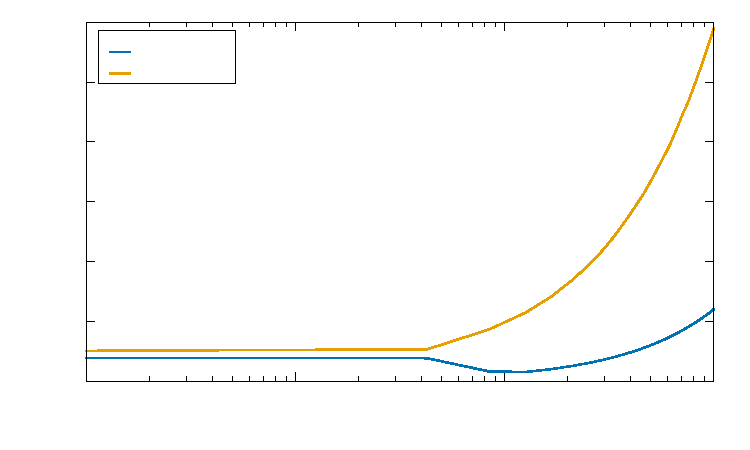
\includegraphics{graf21}}%
    \gplfronttext
  \end{picture}%
\endgroup
} 
    \resizebox{0.32\textwidth}{!}{% GNUPLOT: LaTeX picture with Postscript
\begingroup
  \makeatletter
  \providecommand\color[2][]{%
    \GenericError{(gnuplot) \space\space\space\@spaces}{%
      Package color not loaded in conjunction with
      terminal option `colourtext'%
    }{See the gnuplot documentation for explanation.%
    }{Either use 'blacktext' in gnuplot or load the package
      color.sty in LaTeX.}%
    \renewcommand\color[2][]{}%
  }%
  \providecommand\includegraphics[2][]{%
    \GenericError{(gnuplot) \space\space\space\@spaces}{%
      Package graphicx or graphics not loaded%
    }{See the gnuplot documentation for explanation.%
    }{The gnuplot epslatex terminal needs graphicx.sty or graphics.sty.}%
    \renewcommand\includegraphics[2][]{}%
  }%
  \providecommand\rotatebox[2]{#2}%
  \@ifundefined{ifGPcolor}{%
    \newif\ifGPcolor
    \GPcolortrue
  }{}%
  \@ifundefined{ifGPblacktext}{%
    \newif\ifGPblacktext
    \GPblacktexttrue
  }{}%
  % define a \g@addto@macro without @ in the name:
  \let\gplgaddtomacro\g@addto@macro
  % define empty templates for all commands taking text:
  \gdef\gplbacktext{}%
  \gdef\gplfronttext{}%
  \makeatother
  \ifGPblacktext
    % no textcolor at all
    \def\colorrgb#1{}%
    \def\colorgray#1{}%
  \else
    % gray or color?
    \ifGPcolor
      \def\colorrgb#1{\color[rgb]{#1}}%
      \def\colorgray#1{\color[gray]{#1}}%
      \expandafter\def\csname LTw\endcsname{\color{white}}%
      \expandafter\def\csname LTb\endcsname{\color{black}}%
      \expandafter\def\csname LTa\endcsname{\color{black}}%
      \expandafter\def\csname LT0\endcsname{\color[rgb]{1,0,0}}%
      \expandafter\def\csname LT1\endcsname{\color[rgb]{0,1,0}}%
      \expandafter\def\csname LT2\endcsname{\color[rgb]{0,0,1}}%
      \expandafter\def\csname LT3\endcsname{\color[rgb]{1,0,1}}%
      \expandafter\def\csname LT4\endcsname{\color[rgb]{0,1,1}}%
      \expandafter\def\csname LT5\endcsname{\color[rgb]{1,1,0}}%
      \expandafter\def\csname LT6\endcsname{\color[rgb]{0,0,0}}%
      \expandafter\def\csname LT7\endcsname{\color[rgb]{1,0.3,0}}%
      \expandafter\def\csname LT8\endcsname{\color[rgb]{0.5,0.5,0.5}}%
    \else
      % gray
      \def\colorrgb#1{\color{black}}%
      \def\colorgray#1{\color[gray]{#1}}%
      \expandafter\def\csname LTw\endcsname{\color{white}}%
      \expandafter\def\csname LTb\endcsname{\color{black}}%
      \expandafter\def\csname LTa\endcsname{\color{black}}%
      \expandafter\def\csname LT0\endcsname{\color{black}}%
      \expandafter\def\csname LT1\endcsname{\color{black}}%
      \expandafter\def\csname LT2\endcsname{\color{black}}%
      \expandafter\def\csname LT3\endcsname{\color{black}}%
      \expandafter\def\csname LT4\endcsname{\color{black}}%
      \expandafter\def\csname LT5\endcsname{\color{black}}%
      \expandafter\def\csname LT6\endcsname{\color{black}}%
      \expandafter\def\csname LT7\endcsname{\color{black}}%
      \expandafter\def\csname LT8\endcsname{\color{black}}%
    \fi
  \fi
    \setlength{\unitlength}{0.0500bp}%
    \ifx\gptboxheight\undefined%
      \newlength{\gptboxheight}%
      \newlength{\gptboxwidth}%
      \newsavebox{\gptboxtext}%
    \fi%
    \setlength{\fboxrule}{0.5pt}%
    \setlength{\fboxsep}{1pt}%
\begin{picture}(7200.00,5040.00)%
    \gplgaddtomacro\gplbacktext{%
    }%
    \gplgaddtomacro\gplfronttext{%
      \csname LTb\endcsname%%
      \put(3566,4709){\makebox(0,0){\strut{}$T=3$}}%
    }%
    \gplbacktext
    \put(0,0){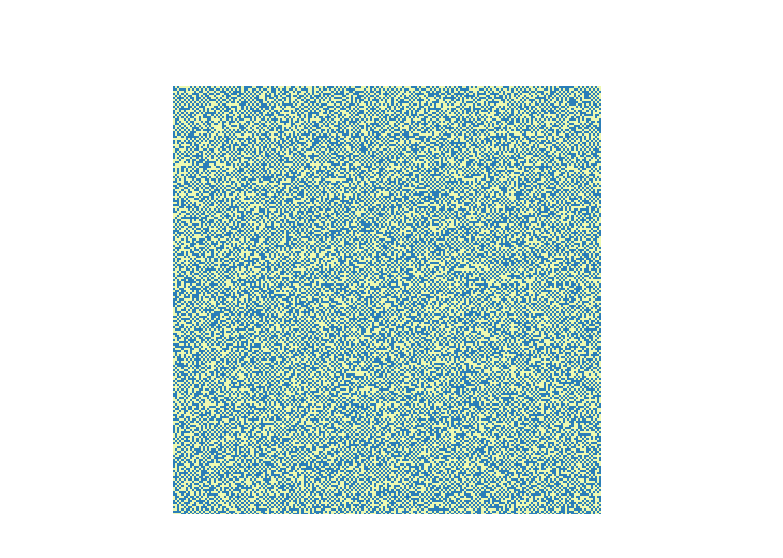
\includegraphics{graf22}}%
    \gplfronttext
  \end{picture}%
\endgroup
} 
    \caption{Končna stanja antiferomagneta pri različnih temperaturah.}
    \label{slika5}
\end{figure}
Za izračun povprečne energije in magnetizacije, vzamemo $10 \times 10$ spinski sistem
in pri vsaki temperaturi $100--$krat izračunamo energijo in magnetizacijo sistema. To
naredimo pri treh različnih vrednostih polja $H=\{ 0, 0.25, 0.5 \}$. Pričakovano 
graf~\ref{slika6} energije raste z~naraščanjem temperature. Magnetizacija sistema je 
najvišja pri temperaturi $T=0$, pri temperaturi prehoda pa pade na nič -- spini niso več 
vsi obrnjeni v~isto smer. Ob prisotnosti zunanjega polja je ta preskok širši. Pri 
specifični toploti imamo pri ob odsotnosti zunanjega polja $H=0$ vrh ravno pri označeni 
kritični temperaturi $T_c \approx 2.27$, ko pa vključimo magnetno polje se ta prehod 
premakne proti višjim temperaturam. To potrdimo tudi z~grafom magnetne susceptibilnosti.
Obe količini po prehodu padeta nazaj na ničlo.
\begin{figure}[H] 
    \centering 
    \resizebox{0.49\textwidth}{!}{% GNUPLOT: LaTeX picture with Postscript
\begingroup
  \makeatletter
  \providecommand\color[2][]{%
    \GenericError{(gnuplot) \space\space\space\@spaces}{%
      Package color not loaded in conjunction with
      terminal option `colourtext'%
    }{See the gnuplot documentation for explanation.%
    }{Either use 'blacktext' in gnuplot or load the package
      color.sty in LaTeX.}%
    \renewcommand\color[2][]{}%
  }%
  \providecommand\includegraphics[2][]{%
    \GenericError{(gnuplot) \space\space\space\@spaces}{%
      Package graphicx or graphics not loaded%
    }{See the gnuplot documentation for explanation.%
    }{The gnuplot epslatex terminal needs graphicx.sty or graphics.sty.}%
    \renewcommand\includegraphics[2][]{}%
  }%
  \providecommand\rotatebox[2]{#2}%
  \@ifundefined{ifGPcolor}{%
    \newif\ifGPcolor
    \GPcolortrue
  }{}%
  \@ifundefined{ifGPblacktext}{%
    \newif\ifGPblacktext
    \GPblacktexttrue
  }{}%
  % define a \g@addto@macro without @ in the name:
  \let\gplgaddtomacro\g@addto@macro
  % define empty templates for all commands taking text:
  \gdef\gplbacktext{}%
  \gdef\gplfronttext{}%
  \makeatother
  \ifGPblacktext
    % no textcolor at all
    \def\colorrgb#1{}%
    \def\colorgray#1{}%
  \else
    % gray or color?
    \ifGPcolor
      \def\colorrgb#1{\color[rgb]{#1}}%
      \def\colorgray#1{\color[gray]{#1}}%
      \expandafter\def\csname LTw\endcsname{\color{white}}%
      \expandafter\def\csname LTb\endcsname{\color{black}}%
      \expandafter\def\csname LTa\endcsname{\color{black}}%
      \expandafter\def\csname LT0\endcsname{\color[rgb]{1,0,0}}%
      \expandafter\def\csname LT1\endcsname{\color[rgb]{0,1,0}}%
      \expandafter\def\csname LT2\endcsname{\color[rgb]{0,0,1}}%
      \expandafter\def\csname LT3\endcsname{\color[rgb]{1,0,1}}%
      \expandafter\def\csname LT4\endcsname{\color[rgb]{0,1,1}}%
      \expandafter\def\csname LT5\endcsname{\color[rgb]{1,1,0}}%
      \expandafter\def\csname LT6\endcsname{\color[rgb]{0,0,0}}%
      \expandafter\def\csname LT7\endcsname{\color[rgb]{1,0.3,0}}%
      \expandafter\def\csname LT8\endcsname{\color[rgb]{0.5,0.5,0.5}}%
    \else
      % gray
      \def\colorrgb#1{\color{black}}%
      \def\colorgray#1{\color[gray]{#1}}%
      \expandafter\def\csname LTw\endcsname{\color{white}}%
      \expandafter\def\csname LTb\endcsname{\color{black}}%
      \expandafter\def\csname LTa\endcsname{\color{black}}%
      \expandafter\def\csname LT0\endcsname{\color{black}}%
      \expandafter\def\csname LT1\endcsname{\color{black}}%
      \expandafter\def\csname LT2\endcsname{\color{black}}%
      \expandafter\def\csname LT3\endcsname{\color{black}}%
      \expandafter\def\csname LT4\endcsname{\color{black}}%
      \expandafter\def\csname LT5\endcsname{\color{black}}%
      \expandafter\def\csname LT6\endcsname{\color{black}}%
      \expandafter\def\csname LT7\endcsname{\color{black}}%
      \expandafter\def\csname LT8\endcsname{\color{black}}%
    \fi
  \fi
    \setlength{\unitlength}{0.0500bp}%
    \ifx\gptboxheight\undefined%
      \newlength{\gptboxheight}%
      \newlength{\gptboxwidth}%
      \newsavebox{\gptboxtext}%
    \fi%
    \setlength{\fboxrule}{0.5pt}%
    \setlength{\fboxsep}{1pt}%
\begin{picture}(7200.00,5040.00)%
    \gplgaddtomacro\gplbacktext{%
      \csname LTb\endcsname%%
      \put(946,704){\makebox(0,0)[r]{\strut{}$-4.5$}}%
      \put(946,1527){\makebox(0,0)[r]{\strut{}$-4$}}%
      \put(946,2350){\makebox(0,0)[r]{\strut{}$-3.5$}}%
      \put(946,3173){\makebox(0,0)[r]{\strut{}$-3$}}%
      \put(946,3996){\makebox(0,0)[r]{\strut{}$-2.5$}}%
      \put(946,4819){\makebox(0,0)[r]{\strut{}$-2$}}%
      \put(1078,484){\makebox(0,0){\strut{}$0$}}%
      \put(1651,484){\makebox(0,0){\strut{}$1$}}%
      \put(2223,484){\makebox(0,0){\strut{}$2$}}%
      \put(2796,484){\makebox(0,0){\strut{}$3$}}%
      \put(3368,484){\makebox(0,0){\strut{}$4$}}%
      \put(3941,484){\makebox(0,0){\strut{}$5$}}%
      \put(4513,484){\makebox(0,0){\strut{}$6$}}%
      \put(5086,484){\makebox(0,0){\strut{}$7$}}%
      \put(5658,484){\makebox(0,0){\strut{}$8$}}%
      \put(6231,484){\makebox(0,0){\strut{}$9$}}%
      \put(6803,484){\makebox(0,0){\strut{}$10$}}%
    }%
    \gplgaddtomacro\gplfronttext{%
      \csname LTb\endcsname%%
      \put(209,2761){\rotatebox{-270}{\makebox(0,0){\strut{}$\langle E\rangle$}}}%
      \put(3940,154){\makebox(0,0){\strut{}$T$}}%
      \csname LTb\endcsname%%
      \put(1669,4184){\makebox(0,0)[l]{\strut{}$H=0$}}%
      \csname LTb\endcsname%%
      \put(1669,4404){\makebox(0,0)[l]{\strut{}$H=0.25$}}%
      \csname LTb\endcsname%%
      \put(1669,4624){\makebox(0,0)[l]{\strut{}$H=0.5$}}%
    }%
    \gplbacktext
    \put(0,0){\includegraphics{graf23}}%
    \gplfronttext
  \end{picture}%
\endgroup
} 
    \resizebox{0.49\textwidth}{!}{% GNUPLOT: LaTeX picture with Postscript
\begingroup
  \makeatletter
  \providecommand\color[2][]{%
    \GenericError{(gnuplot) \space\space\space\@spaces}{%
      Package color not loaded in conjunction with
      terminal option `colourtext'%
    }{See the gnuplot documentation for explanation.%
    }{Either use 'blacktext' in gnuplot or load the package
      color.sty in LaTeX.}%
    \renewcommand\color[2][]{}%
  }%
  \providecommand\includegraphics[2][]{%
    \GenericError{(gnuplot) \space\space\space\@spaces}{%
      Package graphicx or graphics not loaded%
    }{See the gnuplot documentation for explanation.%
    }{The gnuplot epslatex terminal needs graphicx.sty or graphics.sty.}%
    \renewcommand\includegraphics[2][]{}%
  }%
  \providecommand\rotatebox[2]{#2}%
  \@ifundefined{ifGPcolor}{%
    \newif\ifGPcolor
    \GPcolortrue
  }{}%
  \@ifundefined{ifGPblacktext}{%
    \newif\ifGPblacktext
    \GPblacktexttrue
  }{}%
  % define a \g@addto@macro without @ in the name:
  \let\gplgaddtomacro\g@addto@macro
  % define empty templates for all commands taking text:
  \gdef\gplbacktext{}%
  \gdef\gplfronttext{}%
  \makeatother
  \ifGPblacktext
    % no textcolor at all
    \def\colorrgb#1{}%
    \def\colorgray#1{}%
  \else
    % gray or color?
    \ifGPcolor
      \def\colorrgb#1{\color[rgb]{#1}}%
      \def\colorgray#1{\color[gray]{#1}}%
      \expandafter\def\csname LTw\endcsname{\color{white}}%
      \expandafter\def\csname LTb\endcsname{\color{black}}%
      \expandafter\def\csname LTa\endcsname{\color{black}}%
      \expandafter\def\csname LT0\endcsname{\color[rgb]{1,0,0}}%
      \expandafter\def\csname LT1\endcsname{\color[rgb]{0,1,0}}%
      \expandafter\def\csname LT2\endcsname{\color[rgb]{0,0,1}}%
      \expandafter\def\csname LT3\endcsname{\color[rgb]{1,0,1}}%
      \expandafter\def\csname LT4\endcsname{\color[rgb]{0,1,1}}%
      \expandafter\def\csname LT5\endcsname{\color[rgb]{1,1,0}}%
      \expandafter\def\csname LT6\endcsname{\color[rgb]{0,0,0}}%
      \expandafter\def\csname LT7\endcsname{\color[rgb]{1,0.3,0}}%
      \expandafter\def\csname LT8\endcsname{\color[rgb]{0.5,0.5,0.5}}%
    \else
      % gray
      \def\colorrgb#1{\color{black}}%
      \def\colorgray#1{\color[gray]{#1}}%
      \expandafter\def\csname LTw\endcsname{\color{white}}%
      \expandafter\def\csname LTb\endcsname{\color{black}}%
      \expandafter\def\csname LTa\endcsname{\color{black}}%
      \expandafter\def\csname LT0\endcsname{\color{black}}%
      \expandafter\def\csname LT1\endcsname{\color{black}}%
      \expandafter\def\csname LT2\endcsname{\color{black}}%
      \expandafter\def\csname LT3\endcsname{\color{black}}%
      \expandafter\def\csname LT4\endcsname{\color{black}}%
      \expandafter\def\csname LT5\endcsname{\color{black}}%
      \expandafter\def\csname LT6\endcsname{\color{black}}%
      \expandafter\def\csname LT7\endcsname{\color{black}}%
      \expandafter\def\csname LT8\endcsname{\color{black}}%
    \fi
  \fi
    \setlength{\unitlength}{0.0500bp}%
    \ifx\gptboxheight\undefined%
      \newlength{\gptboxheight}%
      \newlength{\gptboxwidth}%
      \newsavebox{\gptboxtext}%
    \fi%
    \setlength{\fboxrule}{0.5pt}%
    \setlength{\fboxsep}{1pt}%
\begin{picture}(7200.00,5040.00)%
    \gplgaddtomacro\gplbacktext{%
      \csname LTb\endcsname%%
      \put(1078,704){\makebox(0,0)[r]{\strut{}$0$}}%
      \put(1078,1527){\makebox(0,0)[r]{\strut{}$0.003$}}%
      \put(1078,2350){\makebox(0,0)[r]{\strut{}$0.006$}}%
      \put(1078,3173){\makebox(0,0)[r]{\strut{}$0.009$}}%
      \put(1078,3996){\makebox(0,0)[r]{\strut{}$0.012$}}%
      \put(1078,4819){\makebox(0,0)[r]{\strut{}$0.015$}}%
      \put(1210,484){\makebox(0,0){\strut{}$0$}}%
      \put(1769,484){\makebox(0,0){\strut{}$1$}}%
      \put(2329,484){\makebox(0,0){\strut{}$2$}}%
      \put(2888,484){\makebox(0,0){\strut{}$3$}}%
      \put(3447,484){\makebox(0,0){\strut{}$4$}}%
      \put(4007,484){\makebox(0,0){\strut{}$5$}}%
      \put(4566,484){\makebox(0,0){\strut{}$6$}}%
      \put(5125,484){\makebox(0,0){\strut{}$7$}}%
      \put(5684,484){\makebox(0,0){\strut{}$8$}}%
      \put(6244,484){\makebox(0,0){\strut{}$9$}}%
      \put(6803,484){\makebox(0,0){\strut{}$10$}}%
    }%
    \gplgaddtomacro\gplfronttext{%
      \csname LTb\endcsname%%
      \put(209,2761){\rotatebox{-270}{\makebox(0,0){\strut{}$c$}}}%
      \put(4006,154){\makebox(0,0){\strut{}$T$}}%
      \csname LTb\endcsname%%
      \put(5747,4184){\makebox(0,0)[l]{\strut{}$H=0$}}%
      \csname LTb\endcsname%%
      \put(5747,4404){\makebox(0,0)[l]{\strut{}$H=0.25$}}%
      \csname LTb\endcsname%%
      \put(5747,4624){\makebox(0,0)[l]{\strut{}$H=0.5$}}%
    }%
    \gplbacktext
    \put(0,0){\includegraphics{graf24}}%
    \gplfronttext
  \end{picture}%
\endgroup
} 

    \resizebox{0.49\textwidth}{!}{% GNUPLOT: LaTeX picture with Postscript
\begingroup
  \makeatletter
  \providecommand\color[2][]{%
    \GenericError{(gnuplot) \space\space\space\@spaces}{%
      Package color not loaded in conjunction with
      terminal option `colourtext'%
    }{See the gnuplot documentation for explanation.%
    }{Either use 'blacktext' in gnuplot or load the package
      color.sty in LaTeX.}%
    \renewcommand\color[2][]{}%
  }%
  \providecommand\includegraphics[2][]{%
    \GenericError{(gnuplot) \space\space\space\@spaces}{%
      Package graphicx or graphics not loaded%
    }{See the gnuplot documentation for explanation.%
    }{The gnuplot epslatex terminal needs graphicx.sty or graphics.sty.}%
    \renewcommand\includegraphics[2][]{}%
  }%
  \providecommand\rotatebox[2]{#2}%
  \@ifundefined{ifGPcolor}{%
    \newif\ifGPcolor
    \GPcolortrue
  }{}%
  \@ifundefined{ifGPblacktext}{%
    \newif\ifGPblacktext
    \GPblacktexttrue
  }{}%
  % define a \g@addto@macro without @ in the name:
  \let\gplgaddtomacro\g@addto@macro
  % define empty templates for all commands taking text:
  \gdef\gplbacktext{}%
  \gdef\gplfronttext{}%
  \makeatother
  \ifGPblacktext
    % no textcolor at all
    \def\colorrgb#1{}%
    \def\colorgray#1{}%
  \else
    % gray or color?
    \ifGPcolor
      \def\colorrgb#1{\color[rgb]{#1}}%
      \def\colorgray#1{\color[gray]{#1}}%
      \expandafter\def\csname LTw\endcsname{\color{white}}%
      \expandafter\def\csname LTb\endcsname{\color{black}}%
      \expandafter\def\csname LTa\endcsname{\color{black}}%
      \expandafter\def\csname LT0\endcsname{\color[rgb]{1,0,0}}%
      \expandafter\def\csname LT1\endcsname{\color[rgb]{0,1,0}}%
      \expandafter\def\csname LT2\endcsname{\color[rgb]{0,0,1}}%
      \expandafter\def\csname LT3\endcsname{\color[rgb]{1,0,1}}%
      \expandafter\def\csname LT4\endcsname{\color[rgb]{0,1,1}}%
      \expandafter\def\csname LT5\endcsname{\color[rgb]{1,1,0}}%
      \expandafter\def\csname LT6\endcsname{\color[rgb]{0,0,0}}%
      \expandafter\def\csname LT7\endcsname{\color[rgb]{1,0.3,0}}%
      \expandafter\def\csname LT8\endcsname{\color[rgb]{0.5,0.5,0.5}}%
    \else
      % gray
      \def\colorrgb#1{\color{black}}%
      \def\colorgray#1{\color[gray]{#1}}%
      \expandafter\def\csname LTw\endcsname{\color{white}}%
      \expandafter\def\csname LTb\endcsname{\color{black}}%
      \expandafter\def\csname LTa\endcsname{\color{black}}%
      \expandafter\def\csname LT0\endcsname{\color{black}}%
      \expandafter\def\csname LT1\endcsname{\color{black}}%
      \expandafter\def\csname LT2\endcsname{\color{black}}%
      \expandafter\def\csname LT3\endcsname{\color{black}}%
      \expandafter\def\csname LT4\endcsname{\color{black}}%
      \expandafter\def\csname LT5\endcsname{\color{black}}%
      \expandafter\def\csname LT6\endcsname{\color{black}}%
      \expandafter\def\csname LT7\endcsname{\color{black}}%
      \expandafter\def\csname LT8\endcsname{\color{black}}%
    \fi
  \fi
    \setlength{\unitlength}{0.0500bp}%
    \ifx\gptboxheight\undefined%
      \newlength{\gptboxheight}%
      \newlength{\gptboxwidth}%
      \newsavebox{\gptboxtext}%
    \fi%
    \setlength{\fboxrule}{0.5pt}%
    \setlength{\fboxsep}{1pt}%
\begin{picture}(7200.00,5040.00)%
    \gplgaddtomacro\gplbacktext{%
      \csname LTb\endcsname%%
      \put(946,704){\makebox(0,0)[r]{\strut{}$-0.2$}}%
      \put(946,1390){\makebox(0,0)[r]{\strut{}$0$}}%
      \put(946,2076){\makebox(0,0)[r]{\strut{}$0.2$}}%
      \put(946,2762){\makebox(0,0)[r]{\strut{}$0.4$}}%
      \put(946,3447){\makebox(0,0)[r]{\strut{}$0.6$}}%
      \put(946,4133){\makebox(0,0)[r]{\strut{}$0.8$}}%
      \put(946,4819){\makebox(0,0)[r]{\strut{}$1$}}%
      \put(1078,484){\makebox(0,0){\strut{}$0$}}%
      \put(1651,484){\makebox(0,0){\strut{}$1$}}%
      \put(2223,484){\makebox(0,0){\strut{}$2$}}%
      \put(2796,484){\makebox(0,0){\strut{}$3$}}%
      \put(3368,484){\makebox(0,0){\strut{}$4$}}%
      \put(3941,484){\makebox(0,0){\strut{}$5$}}%
      \put(4513,484){\makebox(0,0){\strut{}$6$}}%
      \put(5086,484){\makebox(0,0){\strut{}$7$}}%
      \put(5658,484){\makebox(0,0){\strut{}$8$}}%
      \put(6231,484){\makebox(0,0){\strut{}$9$}}%
      \put(6803,484){\makebox(0,0){\strut{}$10$}}%
    }%
    \gplgaddtomacro\gplfronttext{%
      \csname LTb\endcsname%%
      \put(209,2761){\rotatebox{-270}{\makebox(0,0){\strut{}$\langle S\rangle$}}}%
      \put(3940,154){\makebox(0,0){\strut{}$T$}}%
      \csname LTb\endcsname%%
      \put(5747,4184){\makebox(0,0)[l]{\strut{}$H=0$}}%
      \csname LTb\endcsname%%
      \put(5747,4404){\makebox(0,0)[l]{\strut{}$H=0.25$}}%
      \csname LTb\endcsname%%
      \put(5747,4624){\makebox(0,0)[l]{\strut{}$H=0.5$}}%
    }%
    \gplbacktext
    \put(0,0){\includegraphics{graf25}}%
    \gplfronttext
  \end{picture}%
\endgroup
} 
    \resizebox{0.49\textwidth}{!}{% GNUPLOT: LaTeX picture with Postscript
\begingroup
  \makeatletter
  \providecommand\color[2][]{%
    \GenericError{(gnuplot) \space\space\space\@spaces}{%
      Package color not loaded in conjunction with
      terminal option `colourtext'%
    }{See the gnuplot documentation for explanation.%
    }{Either use 'blacktext' in gnuplot or load the package
      color.sty in LaTeX.}%
    \renewcommand\color[2][]{}%
  }%
  \providecommand\includegraphics[2][]{%
    \GenericError{(gnuplot) \space\space\space\@spaces}{%
      Package graphicx or graphics not loaded%
    }{See the gnuplot documentation for explanation.%
    }{The gnuplot epslatex terminal needs graphicx.sty or graphics.sty.}%
    \renewcommand\includegraphics[2][]{}%
  }%
  \providecommand\rotatebox[2]{#2}%
  \@ifundefined{ifGPcolor}{%
    \newif\ifGPcolor
    \GPcolortrue
  }{}%
  \@ifundefined{ifGPblacktext}{%
    \newif\ifGPblacktext
    \GPblacktexttrue
  }{}%
  % define a \g@addto@macro without @ in the name:
  \let\gplgaddtomacro\g@addto@macro
  % define empty templates for all commands taking text:
  \gdef\gplbacktext{}%
  \gdef\gplfronttext{}%
  \makeatother
  \ifGPblacktext
    % no textcolor at all
    \def\colorrgb#1{}%
    \def\colorgray#1{}%
  \else
    % gray or color?
    \ifGPcolor
      \def\colorrgb#1{\color[rgb]{#1}}%
      \def\colorgray#1{\color[gray]{#1}}%
      \expandafter\def\csname LTw\endcsname{\color{white}}%
      \expandafter\def\csname LTb\endcsname{\color{black}}%
      \expandafter\def\csname LTa\endcsname{\color{black}}%
      \expandafter\def\csname LT0\endcsname{\color[rgb]{1,0,0}}%
      \expandafter\def\csname LT1\endcsname{\color[rgb]{0,1,0}}%
      \expandafter\def\csname LT2\endcsname{\color[rgb]{0,0,1}}%
      \expandafter\def\csname LT3\endcsname{\color[rgb]{1,0,1}}%
      \expandafter\def\csname LT4\endcsname{\color[rgb]{0,1,1}}%
      \expandafter\def\csname LT5\endcsname{\color[rgb]{1,1,0}}%
      \expandafter\def\csname LT6\endcsname{\color[rgb]{0,0,0}}%
      \expandafter\def\csname LT7\endcsname{\color[rgb]{1,0.3,0}}%
      \expandafter\def\csname LT8\endcsname{\color[rgb]{0.5,0.5,0.5}}%
    \else
      % gray
      \def\colorrgb#1{\color{black}}%
      \def\colorgray#1{\color[gray]{#1}}%
      \expandafter\def\csname LTw\endcsname{\color{white}}%
      \expandafter\def\csname LTb\endcsname{\color{black}}%
      \expandafter\def\csname LTa\endcsname{\color{black}}%
      \expandafter\def\csname LT0\endcsname{\color{black}}%
      \expandafter\def\csname LT1\endcsname{\color{black}}%
      \expandafter\def\csname LT2\endcsname{\color{black}}%
      \expandafter\def\csname LT3\endcsname{\color{black}}%
      \expandafter\def\csname LT4\endcsname{\color{black}}%
      \expandafter\def\csname LT5\endcsname{\color{black}}%
      \expandafter\def\csname LT6\endcsname{\color{black}}%
      \expandafter\def\csname LT7\endcsname{\color{black}}%
      \expandafter\def\csname LT8\endcsname{\color{black}}%
    \fi
  \fi
    \setlength{\unitlength}{0.0500bp}%
    \ifx\gptboxheight\undefined%
      \newlength{\gptboxheight}%
      \newlength{\gptboxwidth}%
      \newsavebox{\gptboxtext}%
    \fi%
    \setlength{\fboxrule}{0.5pt}%
    \setlength{\fboxsep}{1pt}%
\begin{picture}(7200.00,5040.00)%
    \gplgaddtomacro\gplbacktext{%
      \csname LTb\endcsname%%
      \put(1078,704){\makebox(0,0)[r]{\strut{}$0$}}%
      \put(1078,1390){\makebox(0,0)[r]{\strut{}$0.005$}}%
      \put(1078,2076){\makebox(0,0)[r]{\strut{}$0.01$}}%
      \put(1078,2762){\makebox(0,0)[r]{\strut{}$0.015$}}%
      \put(1078,3447){\makebox(0,0)[r]{\strut{}$0.02$}}%
      \put(1078,4133){\makebox(0,0)[r]{\strut{}$0.025$}}%
      \put(1078,4819){\makebox(0,0)[r]{\strut{}$0.03$}}%
      \put(1210,484){\makebox(0,0){\strut{}$0$}}%
      \put(1769,484){\makebox(0,0){\strut{}$1$}}%
      \put(2329,484){\makebox(0,0){\strut{}$2$}}%
      \put(2888,484){\makebox(0,0){\strut{}$3$}}%
      \put(3447,484){\makebox(0,0){\strut{}$4$}}%
      \put(4007,484){\makebox(0,0){\strut{}$5$}}%
      \put(4566,484){\makebox(0,0){\strut{}$6$}}%
      \put(5125,484){\makebox(0,0){\strut{}$7$}}%
      \put(5684,484){\makebox(0,0){\strut{}$8$}}%
      \put(6244,484){\makebox(0,0){\strut{}$9$}}%
      \put(6803,484){\makebox(0,0){\strut{}$10$}}%
    }%
    \gplgaddtomacro\gplfronttext{%
      \csname LTb\endcsname%%
      \put(209,2761){\rotatebox{-270}{\makebox(0,0){\strut{}$\chi$}}}%
      \put(4006,154){\makebox(0,0){\strut{}$T$}}%
      \csname LTb\endcsname%%
      \put(5747,4184){\makebox(0,0)[l]{\strut{}$H=0$}}%
      \csname LTb\endcsname%%
      \put(5747,4404){\makebox(0,0)[l]{\strut{}$H=0.25$}}%
      \csname LTb\endcsname%%
      \put(5747,4624){\makebox(0,0)[l]{\strut{}$H=0.5$}}%
    }%
    \gplbacktext
    \put(0,0){\includegraphics{graf26}}%
    \gplfronttext
  \end{picture}%
\endgroup
} 
    \caption{Energija, specifična toplota, magnetizacija in spinska susceptibilnost 
    feromagnetnega sistema pri različnih parametrih $H$.}
    \label{slika6}
\end{figure}
\end{document}
